\chapter{相似形}

\section{比例线段}
\subsection{比例}\label{subsec:czjh2-6-1}

\begin{enhancedline}

前面,我们学习了全等图形。两个全等图形的形状相同,大小也相同,它们能够完全重合。
我们还常见到这样的一些图形,如国旗上的大五角星和小五角星;
图 \ref{fig:czjh2-6-1} 中我们伟大祖国的两幅大小不同的地图。
这些图形大小虽然不同,但形状却是相同的。

\begin{figure}[htbp]
    \centering
    \includegraphics[width=5cm]{../pic/czjh2-ch6-01.png}
    \caption{}\label{fig:czjh2-6-1}
\end{figure}

为了研究这些形状相同的图形之间的关系,我们需要先研究比例和比例线段。

在小学里,我们学过比例,就是两个比相等的式子。如
\begin{gather*}
    \exdfrac{80}{2} = \exdfrac{240}{6} \quad \text{或} \quad 80:2 = 240:6 \juhao
\end{gather*}

%\qquad $\dfrac{80}{2} = \dfrac{240}{6}$ 或 $80:2 = 240:6$。

如果用字母來表示数,那么比例可以写成如下的形式(只研究所有的字母都不等于零的情形):
\begin{gather*}
    \exdfrac{a}{b} = \exdfrac{c}{d} \quad \text{或} \quad a:b = c:d \juhao
\end{gather*}

在比例中,$a$、$d$ 叫做\zhongdian{比例外项},
$b$、$c$ 叫做\zhongdian{比例内项},
$d$ 叫做 $a$、$b$、$c$ 的\zhongdian{第四比例项}。
如果比例中两个比例内项相等,即比例为
\begin{gather*}
    \exdfrac{a}{b} = \exdfrac{b}{c} \quad \text{或} \quad a:b = b:c
\end{gather*}
时,我们把 $b$ 叫做 $a$ 和 $c$ 的\zhongdian{比例中项}。

在比例 $\exdfrac{a}{b} = \exdfrac{c}{d}$ 的两边同乘以 $bd$,得到
\begin{gather*}
    ad = bc \juhao
\end{gather*}

这个推理步骤就是:

$\because$ \quad $\exdfrac{a}{b} = \exdfrac{c}{d}$,

$\therefore$ \quad $ad = bc$。

为了简明,可以把这个推理步骤写成:
\begin{gather}
    \exdfrac{a}{b} = \exdfrac{c}{d} \tuichu  ad = bc \juhao  \tag{1}
\end{gather}

符号 “$\tuichu$” 读作 “推出”。

在等式 $ad = bc$  的两边同除以 $bd$,又得到 $\exdfrac{a}{b} = \exdfrac{c}{d}$,即
\begin{gather}
    ad = bc  \tuichu  \exdfrac{a}{b} = \exdfrac{c}{d} \juhao  \tag{2}
\end{gather}

(1)、(2) 式合起来表示 $\exdfrac{a}{b} = \exdfrac{c}{d}$ 与 $ad = bc$ 可以
互相推出,这是比例的基本性质。

\begin{dingli}[比例的性质定理]
    $$ \bm{
        \exdfrac{a}{b} = \exdfrac{c}{d} \dengjiayu ad = bc \juhao
    }$$
\end{dingli}

符号 “$\dengjiayu$” 读作“等价于”。它表示从左端可以推出右端,并且从右端也可以推出左端。

\begin{tuilun}[推论]
    $\bm{
        \exdfrac{a}{b} = \exdfrac{b}{c}  \dengjiayu  b^2 = ac \juhao
    }$
\end{tuilun}

根据比例的性质定理,一个比例可以得出多种不同的比例变形。例如,

$\exdfrac{a}{b} = \exdfrac{c}{d}  \tuichu  ad = bc  \tuichu  bc = ad   \tuichu \exdfrac{b}{a} = \exdfrac{d}{c}$。

由于  $ad = bc$ 可以写成  $bc = ad$, $ad = cb$, $cb = da$,… 等七种形式,
所以由 $\exdfrac{a}{b} = \exdfrac{c}{d}$ 又可以得出
$\exdfrac{b}{a} = \exdfrac{d}{c}$,
$\exdfrac{a}{c} = \exdfrac{b}{d}$,
$\exdfrac{c}{d} = \exdfrac{a}{b}$,… 等七种不同形式。

\liti 依据下列各式,求 $a:b$ :

(1)$3a = 4b$;(2)$\exdfrac{a}{5} = \exdfrac{b}{7}$。

\jie (1)$3a = 4b  \tuichu \exdfrac{a}{b} = \exdfrac{4}{3}$;

(2)$\exdfrac{a}{5} = \exdfrac{b}{7}  \tuichu  \exdfrac{a}{b} = \exdfrac{5}{7}$。


下面,我们再学习比例的两个重要性质:

1. \begin{xingzhi}[合比性质]
    \newline\ \hspace*{3em}
    $\bm{
        \exdfrac{a}{b} = \exdfrac{c}{d}  \tuichu \dfrac{a \pm b}{b} = \dfrac{c \pm d}{d} \juhao
    }$
\end{xingzhi}

\zhengming $\begin{aligned}[t]
    \exdfrac{a}{b} = \exdfrac{c}{d}  &\tuichu  \exdfrac{a}{b} \pm 1 = \exdfrac{c}{d} \pm 1 \\
                                     &\tuichu  \dfrac{a \pm b}{b} = \dfrac{c \pm d}{d} \juhao
\end{aligned}$


2. \begin{xingzhi}[等比性质]
    \newline\ \hspace*{3em}
    $\begin{aligned}[t]
        \bm{\exdfrac{a}{b}} &= \bm{\exdfrac{c}{d} = \cdots = \exdfrac{m}{n} \; (b + d + \cdots + n \neq 0)} \\
                            & \bm{\tuichu \dfrac{a  + c + \cdots + m}{b + d + \cdots + n} = \exdfrac{a}{b} \juhao}
    \end{aligned}$
\end{xingzhi}

\zhengming 设 $\exdfrac{a}{b} = \exdfrac{c}{d} = \cdots = \exdfrac{m}{n} = k$,
那么 $a = bk$, $c = dk$,…, $m = nk$。

$\begin{aligned}[t]
    \dfrac{a + c + \cdots + m}{b + d + \cdots + n}
        &= \dfrac{bk + dk + \cdots + nk}{b + d + \cdots + n} \\
        &= \dfrac{(b + d + \cdots + n)k}{b + d + \cdots + n} = k = \exdfrac{a}{b} \juhao
\end{aligned}$



\liti (1)已知: $\dfrac{a - b}{b} = \exdfrac{3}{8}$。求证  $\exdfrac{a}{b} = \dfrac{11}{8}$;

(2)已知: $\exdfrac{a}{b} = \exdfrac{c}{d} \; (b \pm d \neq 0)$。
求证: $\dfrac{a + c}{a - c} = \dfrac{b + d}{b - d}$。

\zhengming (1) $\begin{aligned}[t]
    \dfrac{a - b}{b} = \exdfrac{3}{8}
        &\tuichu \dfrac{a - b + b}{8} = \dfrac{3 + 8}{8} \\
        &\tuichu \exdfrac{a}{b} = \dfrac{11}{8} \fenhao
\end{aligned}$


(2)$\begin{aligned}[t]
    \exdfrac{a}{b} = \exdfrac{c}{d}
        &\tuichu \left\{
                \begin{gathered}
                    \dfrac{a + c}{b + d} = \exdfrac{a}{b} \\
                    \dfrac{a - c}{b - d} = \exdfrac{a}{b} \\
                \end{gathered}
            \right\} \tuichu \dfrac{a + c}{b + d} = \dfrac{a - c}{b - d} \\
        &\tuichu \dfrac{a + c}{a - c} = \dfrac{b + d}{b - d} \juhao
\end{aligned}$


\liti 已知: $\exdfrac{a}{b}  = \exdfrac{c}{d} = \exdfrac{e}{f} = 3$,
$b + d + f = 4$。 求 $a + c + e$。

\jie $\begin{aligned}[t]
    \exdfrac{a}{b}  = \exdfrac{c}{d} = \exdfrac{e}{f} = 3
        & \tuichu \dfrac{a + c + e}{b + d + f} = 3 \\
        & \left.\begin{aligned}
                \tuichu a + c + e = 3 (b + d + f) & \\
                b + d + f = 4 &
            \end{aligned} \right\} \\
        & \tuichu a + c + e = 3 \times 4 = 12 \juhao
\end{aligned}$


\begin{lianxi}

\xiaoti{求下列各式中的 $x$:}
\begin{xiaoxiaotis}

    \begin{tblr}{columns={18em, colsep=0pt}}
        \xxt{$4:x = 3:5$;}  & \xxt{$(x + 2):x = 11:9$;} \\
        \xxt{$3:x = x:12$;} & \xxt{$1:x = x:(1 - x)$。}
    \end{tblr}

\end{xiaoxiaotis}


\xiaoti{已知: $\exdfrac{a}{b} = \exdfrac{c}{d}$。写出其他七个比例式,并指出其中
    哪些是以 $a$ 和 $d$ 为外项,以 $b$ 和 $c$ 为内项的比例式,
    哪些是以 $b$ 和 $c$ 为外项,以 $a$ 和 $d$ 为内项的比例式。
}


\xiaoti{从下列各式求 $x:y$:}
\begin{xiaoxiaotis}

    \begin{tblr}{columns={12em, colsep=0pt}}
        \xxt{$3y = 4x$;} & \xxt{$3:2 = y:x$;} & \xxt{$7:x = 4:y$;} \\
        \xxt{$m:y = n:x$;} & \xxt{$(x+y):y = 8:3$;} & \xxt{$(x-y):y = 1:2$。}
    \end{tblr}

\end{xiaoxiaotis}


\xiaoti{已知 $h$ 是 $e$、$f$、$g$ 的第四比例项,写出比例式。}

\xiaoti{已知: $\exdfrac{a}{b} = \exdfrac{c}{d} = \exdfrac{e}{f} = \exdfrac{5}{7}$。
    求 $\dfrac{2a - c + 7e}{2b - d + 7f}$。
}


\xiaoti{(口答)}
\begin{xiaoxiaotis}

    \xxt{$\exdfrac{a}{b}$ 是不是等于 $\exdfrac{a^2}{b^2}$? 为什么?}

    \xxt{从 $\exdfrac{a}{b} = \exdfrac{c}{d}$ 能不能得出 $\exdfrac{a^2}{b^2} = \exdfrac{c^2}{d^2}$?为什么?}

\end{xiaoxiaotis}


\xiaoti{从下面两个比例可以推出什么结果:}
\begin{xiaoxiaotis}

    \xxt{$b:a = c:b$;}

    \xxt{$b:a = b:c$。}

\end{xiaoxiaotis}

\end{lianxi}
\end{enhancedline}


\subsection{比例线段}\label{subsec:czjh2-6-2}

\begin{enhancedline}

我们先来研究两条线段的比。

在同一单位下,两条线段长度的比叫做这\zhongdian{两条线段的比}。
两条线段  $AB$、$CD$ 的比值为 $k$ 时,可以记作:
$$ \dfrac{AB}{CD} = k  \quad \text{或} \quad  AB:CD = k \juhao $$
因为线段的长度是一个正量,所以两条线段的比值一定是正数。
例如,课本的封面相邻两边 $a$、$b$ 的长度分别是 $18.5 \;\limi$ 和 $13 \;\limi$,那么
$$ \exdfrac{a}{b} = \dfrac{18.5}{13} = \dfrac{37}{26} \quad \text{或} \quad  a:b = 18.5:13 = \dfrac{37}{26} \juhao $$

如果改用米、毫米作为线段的长度单位,那么
\begin{align*}
    & a:b = 0.185:0.130 = \dfrac{37}{26} \fenhao \\
    & a:b = 185:130 = \dfrac{37}{26} \juhao
\end{align*}


由此可知:两条线段的比值与所采用的长度单位没有关系。
因此,下面讨论线段的比时,一般不指明长度单位。
但如果遇到给出的线段长度使用不同的单位时,要先化成同一单位。

\begin{wrapfigure}[11]{r}{6.5cm}
    \centering
    \begin{tikzpicture}
    \pgfmathsetmacro{\a}{3}
    \pgfmathsetmacro{\b}{1.2}
    \pgfmathsetmacro{\c}{2}
    \pgfmathsetmacro{\d}{0.8}

    \begin{scope}
        \tkzDefPoints{0/0/A, \a/0/B, \a/\c/C, 0/\c/D}
        \tkzDrawPolygon(A,B,C,D)
        \tkzDrawSegments[dim={$a$,-10pt,}](A,B)
        \tkzDrawSegments[dim={$c$, 10pt,rotate=90}](A,D)
    \end{scope}

    \begin{scope}[xshift=4cm]
        \tkzDefPoints{0/0/A, \b/0/B, \b/\d/C, 0/\d/D}
        \tkzDrawPolygon(A,B,C,D)
        \tkzDrawSegments[dim={$b$,-10pt,}](A,B)
        \tkzDrawSegments[dim={$d$,-10pt,rotate=90}](B,C)
    \end{scope}
\end{tikzpicture}


    \caption{}\label{fig:czjh2-6-2}
\end{wrapfigure}

如图 \ref{fig:czjh2-6-2},分别度量两个矩形的长 $a$ 和 $b$,宽 $c$ 和 $d$,得
$$ a = 3\;\limi \douhao  b = 12\;\haomi \douhao  c = 2\;\limi \douhao  d = 8\;\haomi \douhao$$
改成用 $\haomi$ 为单位,得 $a = 30\;\haomi$, $c = 20\;\haomi$。可得
$$ \exdfrac{a}{b} = \dfrac{30}{12} = 2.5 \douhao  \quad \exdfrac{c}{d} = \dfrac{20}{8} = 2.5 \juhao $$
于是得
$$ \exdfrac{a}{b} = \exdfrac{c}{d}  \quad \text{或} \quad  a:b = c:d  \juhao $$

在四条线段 $a$、$b$、$c$、$d$ 中,如果 $a$ 和 $b$ 的比等于 $c$ 和 $d$ 的比,
那么,这四条线段叫做\zhongdian{成比例线段}或简称\zhongdian{比例线段}。


\liti 两地的实际距离是 250 m,画在地图上的距离(图距)是 5 cm,图距与实际距离的比($0.05:250$)
就是比例尺 $\left(\dfrac{1}{5000}\right)$。在这样的地图上,图距 $a=8$ cm 的两地 $A$、$B$,
实际距离是多少米?

\jie 根据题意
$$ \dfrac{a}{AB} = \dfrac{1}{5000} \douhao $$

$\therefore$ \quad $AB = 5000 a = 40000 \; (\limi) = 400 \;(\mi) \juhao$

答: $A$、$B$ 两地的实际距离是 400 米。


\begin{wrapfigure}[4]{r}{5cm}
    \centering
    \begin{tikzpicture}
    \tkzDefPoints{0/0/A, 4/0/B}
    \tkzDefPointOnLine[pos=0.618](A,B)  \tkzGetPoint{C}
    \tkzDrawSegments[xianduan={below=0pt}](A,C)
    \tkzDrawSegments[xianduan={below=0pt}](C,B)
    \tkzLabelPoints[above=.5em](A,B,C)
\end{tikzpicture}


    \caption{}\label{fig:czjh2-6-3}
\end{wrapfigure}

\liti 已知线段 $AB=l$, $C$ 是 $AB$ 上的一点(图 \ref{fig:czjh2-6-3}),且 $AC$ 是 $AB$ 和 $BC$ 的比例中项。求 $AC$ 的长。

\jie 设 $AC = x$,那么 $BC = AB - AC = l - x$。

因为 $AC$ 是 $AB$ 和 $BC$ 的比例中项,得
\begin{align*}
    & x^2 = l \, (l - x) \douhao \\
    & x^2 + lx = l^2 = 0 \juhao
\end{align*}

解得 \qquad $x = \dfrac{-l \pm \sqrt{l^2 + 4l^2}}{2}$ ,

$x_1 = \dfrac{-1 + \sqrt{5}}{2} \, l$, $x_2 = \dfrac{-1 - \sqrt{5}}{2} \, l$ (不合题意)。

即 $AC = \dfrac{\sqrt{5} - 1}{2} \, l \approx 0.618 \, l$。

把一条线段($AB$)分成两条线段,使其中较大的线段($AC$)是原线段($AB$)
与较小的线段($BC$)的比例中项,叫做把这条线段\zhongdian{黄金分割}。

在一条线段 $AB$ 上截取这条线段的 $0.618$ 倍得点 $C$,点 $C$ 就是线段 $AB$ 的黄金分割点(近似)。
我们也可以根据勾段定理,利用尺规作图作出 $\sqrt{\left(\exdfrac{l}{2}\right)^2 + l^2}$,
再作出一条线段的黄金分割点。作法如下:

1. 过点 $B$ 作 $BD \perp AB$,使 $BD = \exdfrac{1}{2} AB$(图 \ref{fig:czjh2-6-4})。

\begin{wrapfigure}[5]{r}{6cm}
    \centering
    \begin{tikzpicture}
    \pgfmathsetmacro{\l}{4}

    % 0
    \tkzDefPoints{0/0/A, \l/0/B}
    \tkzDrawSegments(A,B)
    \tkzLabelPoints[left](A)
    \tkzLabelPoints[right](B)

    % 1
    \tkzDefPointOnLine[pos=0.5](A,B)  \tkzGetPoint{d1}
    \tkzDefLine[perpendicular=through B](A,B)  \tkzGetPoint{d2}
    \tkzInterLC(B,d2)(B,d1)  \tkzGetSecondPoint{D}
    \tkzDrawSegment(B,D)
    \tkzLabelPoints[right](D)

    % 2
    \tkzDrawSegment(A,D)
    \tkzInterLC(A,D)(D,B)  \tkzGetFirstPoint{E}
    \tkzDrawArc[towards](D,E)(B)
    \tkzLabelPoints[above](E)

    % 3
    \tkzInterLC(A,B)(A,E)  \tkzGetSecondPoint{C}
    \tkzDrawArc[towards](A,C)(E)
    \tkzLabelPoints[below](C)
\end{tikzpicture}


    \caption{}\label{fig:czjh2-6-4}
\end{wrapfigure}


2. 连结 $AD$,在 $AD$ 上截取 $DE = DB$。

3. 在 $AB$ 上截取 $AC = AE$。

点 $C$ 就是所求的黄金分割点。

这是因为, $\begin{aligned}[t]
    AC &= AE = AD - \dfrac{AB}{2} \\
       &= \sqrt{AB^2 + \left(\dfrac{AB}{2}\right)^2} - \dfrac{AB}{2} \\
       &= \dfrac{\sqrt{5} AB}{2} - \dfrac{AB}{2} = \dfrac{\sqrt{5} - 1}{2} AB \juhao
\end{aligned}$


\begin{lianxi}

\xiaoti{延长线段 $AB$ 到 $C$,使 $BC = AB$。求}
\begin{xiaoxiaotis}

    \threeInLineXxt[12em]{$AC:AB$;}{$AB:BC$;}{$AC:BC$。}

\end{xiaoxiaotis}


\xiaoti{求正方形的对角线和它的一边的比值:}
\begin{xiaoxiaotis}

    \xxt{用根式表示;}
    \xxt{精确到 $0.1$;}
    \xxt{精确到 $0.001$。}

\end{xiaoxiaotis}

\xiaoti{(口答)如图所示的三个矩形中,哪两个矩形的长和宽是成比例的线段?}

\begin{figure}[htbp]
    \centering
    \begin{minipage}[b]{9cm}
        \centering
        \begin{tikzpicture}[scale=0.3]
    \begin{scope}
        \pgfmathsetmacro{\a}{8}
        \pgfmathsetmacro{\b}{6}
        \tkzDefPoints{0/0/A, \a/0/B, \a/\b/C, 0/\b/D}
        \tkzDrawPolygon(A,B,C,D)
        \tkzDrawSegments[dim={$\a$,-10pt,}](A,B)
        \tkzDrawSegments[dim={$\b$, 10pt,rotate=90}](A,D)
    \end{scope}

    \begin{scope}[xshift=11cm]
        \pgfmathsetmacro{\a}{8}
        \pgfmathsetmacro{\b}{4}
        \tkzDefPoints{0/0/A, \a/0/B, \a/\b/C, 0/\b/D}
        \tkzDrawPolygon(A,B,C,D)
        \tkzDrawSegments[dim={$\a$,-10pt,}](A,B)
        \tkzDrawSegments[dim={$\b$, 10pt,rotate=90}](A,D)
    \end{scope}

    \begin{scope}[xshift=22cm]
        \pgfmathsetmacro{\a}{6}
        \pgfmathsetmacro{\b}{4.5}
        \tkzDefPoints{0/0/A, \a/0/B, \a/\b/C, 0/\b/D}
        \tkzDrawPolygon(A,B,C,D)
        \tkzDrawSegments[dim={$\a$,-10pt,}](A,B)
        \tkzDrawSegments[dim={$\b$, 10pt,rotate=90}](A,D)
    \end{scope}
\end{tikzpicture}


        \caption*{(第 3 题)}
    \end{minipage}
    \qquad
    \begin{minipage}[b]{5cm}
        \centering
        \begin{tikzpicture}
    \tkzDefPoints{0/0/B, 3/0/C}
    \tkzInterCC[R](B,4)(C,2.8)  \tkzGetFirstPoint{A}
    \tkzDefPointOnLine[pos=15/40](A,B)  \tkzGetPoint{D}
    \tkzDefLine[parallel=through D](B,C)  \tkzGetPoint{e}
    \tkzInterLL(A,C)(D,e)  \tkzGetPoint{E}

    \tkzDrawPolygon(A,B,C)
    \tkzDrawSegment(D,E)
    \tkzLabelPoints[above](A)
    \tkzLabelPoints[left](B,D)
    \tkzLabelPoints[right](C,E)
\end{tikzpicture}


        \caption*{(第 5 题)}
    \end{minipage}
\end{figure}

\xiaoti{已知:线段 $a = \exdfrac{1}{7} \;\limi$, $b = 4\;\limi$, $c = 28\sqrt{2}\;\limi$。
    求 $a$、$b$、$c$ 的第四比例项。
}

\xiaoti{已知:如图, $\dfrac{AD}{DB} = \dfrac{AE}{EC}$, $AD = 15$, $AB = 40$,$AC = 28$, 求 $AE$ 的长。}

\end{lianxi}
\end{enhancedline}




\xiti
\begin{xiaotis}
\begin{enhancedline}

\xiaoti{烟囱高 30 米,影长 20 米; 竿高 1.5 米,影长 1 米。 物高与影长成比例吗?}

\xiaoti{}%
\begin{xiaoxiaotis}%
    \xxt[\xxtsep]{求等腰直角三角形的直角边与斜边的比;}

    \xxt{求正三角形的高与边长的比。}

\end{xiaoxiaotis}

\xiaoti{把下列各式写成比例的形式:}
\begin{xiaoxiaotis}

    \threeInLineXxt[12em]{$mn = pq$;}{$a^2 = bc$;}{$x = \dfrac{bc}{a}$。}

\end{xiaoxiaotis}


\xiaoti{已知  $\exdfrac{a}{b} = \exdfrac{c}{d}$。}
\begin{xiaoxiaotis}

    \begin{tblr}{columns={18em, colsep=0pt}}
        \xxt{用 $b$、$c$、$d$ 表示 $a$;} & \xxt{用 $a$、$c$、$d$ 表示 $b$。}
    \end{tblr}
\end{xiaoxiaotis}


\xiaoti{图纸上画出的某个零件的长是 32 毫米,如果比例尺是 $1:20$,
    这个零件实际的长是多少?如果比例尺是 $5:1$ 呢?
}

\xiaoti{在相同时刻的物高与影长成比例。如果某建筑物在地面上的影长为 50 米,
    同时,高为 1.5 米的测竿的影长为 2.5 米,那么建筑物的高是多少米?
}

\xiaoti{在两个比例式 $\exdfrac{a}{b} = \exdfrac{c}{d}$ 和 $\dfrac{a'}{b'} = \dfrac{c'}{d'}$ 中,
    如果 $a = a'$,$b = b'$,$c = c'$, 那么 $d$ 和 $d'$  是不是相等?为什么?
}

\xiaoti{已知: $\exdfrac{x}{2} = \exdfrac{y}{3} = \exdfrac{z}{4}$。求}
\begin{xiaoxiaotis}

    \begin{tblr}{columns={12em, colsep=0pt}}
         \xxt{$\dfrac{x + y + z}{x}$;} & \xxt{$\dfrac{x + y + z}{x + y - z}$;} & \xxt{$\dfrac{y + z - x}{z + x - y}$。}
    \end{tblr}
\end{xiaoxiaotis}

\xiaoti{已知: $x:y:z = 3:4:5$, $x + y - z = 6$。 求 $x$、$y$ 和 $z$。\\
    (注:$x:y:z = 3:4:5$ 是 $x:3 = y:4 = z:5$ 的另一种写法。)
}


\xiaoti{}%
\begin{xiaoxiaotis}%
    \xxt[\xxtsep]{求证: $\exdfrac{a}{b} = \exdfrac{c}{d}  \tuichu \dfrac{a + b}{a - b} = \dfrac{c + d}{c - d}$;}

    \xxt{求证: $\exdfrac{a}{b} = \exdfrac{c}{d}  \tuichu  \dfrac{a}{a + b} = \dfrac{c}{c + d}$。}

\end{xiaoxiaotis}


\xiaoti{如图,$\triangle ABC$ 中, $DE \pingxing BC$, $AH \perp BC$, $AH$ 交 $DE$ 于点 $G$。
    已知: $\dfrac{AG}{DE} = \dfrac{AH}{BC}$, 且 $DE = 12$, $BC = 15$, $GH = 6$。 求高 $AH$。
}

\begin{figure}[htbp]
    \centering
    \begin{minipage}[b]{7cm}
        \centering
        \begin{tikzpicture}[scale=0.12]
    \tkzDefPoints{0/0/B, 15/0/C}
    \tkzDefPointOnLine[pos=0.7](B,C)  \tkzGetPoint{H}
    \tkzDefShiftPoint[H](0,6){G}  % GH = 6
    \tkzDefShiftPoint[H](0,30){A} % 计算得到 AH = 30
    \tkzDefLine[parallel=through G](B,C)  \tkzGetPoint{d}
    \tkzInterLL(G,d)(A,B)  \tkzGetPoint{D}
    \tkzInterLL(G,d)(A,C)  \tkzGetPoint{E}

    \tkzDrawPolygon(A,B,C)
    \tkzDrawSegments(D,E  A,H)
    \tkzMarkRightAngle[size=2](C,H,A)
    \tkzLabelPoints[above](A)
    \tkzLabelPoints[left](B,D)
    \tkzLabelPoints[right](C,E)
    \tkzLabelPoints[below](H)
    \tkzLabelPoints[above left](G)

    % \tkzCalcLength(D,E)  \tkzGetLength{de}
    % \tkzLabelSegment(D,E){\de}
\end{tikzpicture}


        \caption*{(第 11 题)}
    \end{minipage}
    \qquad
    \begin{minipage}[b]{7cm}
        \centering
        \begin{tikzpicture}
    \tkzDefPoints{0/0/xa1, 3/0/xa2, 0/1.5/xb1, 3/1.5/xb2, 0/2.5/xc1, 3/2.5/xc2}
    \tkzDefPoints{1.1/3/ya1, 0.5/-0.5/ya2, 1.6/3/yb1, 2.5/-0.5/yb2}

    \tkzInterLL(xc1,xc2)(ya1,ya2)  \tkzGetPoint{A}
    \tkzInterLL(xc1,xc2)(yb1,yb2)  \tkzGetPoint{C}
    \tkzInterLL(xb1,xb2)(ya1,ya2)  \tkzGetPoint{E}
    \tkzInterLL(xb1,xb2)(yb1,yb2)  \tkzGetPoint{F}
    \tkzInterLL(xa1,xa2)(ya1,ya2)  \tkzGetPoint{B}
    \tkzInterLL(xa1,xa2)(yb1,yb2)  \tkzGetPoint{D}

    \tkzDrawSegments(xa1,xa2  xb1,xb2  xc1,xc2)
    \tkzDrawSegments(ya1,ya2  yb1,yb2)
    \tkzLabelPoints[above left](A,B,E)
    \tkzLabelPoints[above right](C,D,F)
\end{tikzpicture}


        \caption*{(第 13 题)}
    \end{minipage}
\end{figure}

\xiaoti{}%
\begin{xiaoxiaotis}%
    \xxt[\xxtsep]{已知: $a = 4$ 厘米, $b = 6$ 厘米, $c = 3$ 厘米。 求 $a$、$b$、$c$ 的第四比例项 $d$;}

    \xxt{已知: $a = 2.4$ 厘米, $c = 5.4$ 厘米。 求 $a$ 和 $c$ 的比例中项 $b$;}

    \xxt{已知: 线段 $a = 1$, $b = \dfrac{\sqrt{5} - 1}{2}$, $c = \dfrac{3 - \sqrt{5}}{2}$。 求证: 线段 $b$ 是 $a$、$c$ 的比例中项。}

\end{xiaoxiaotis}


\xiaoti{已知: 如图, $\dfrac{AE}{EB} = \dfrac{CF}{FD}$。 依据比例的性质证明:}
\begin{xiaoxiaotis}

    \begin{tblr}{columns={12em, colsep=0pt}}
        \xxt{$\dfrac{AE}{CF} = \dfrac{EB}{FD}$;}
            & \xxt{$\dfrac{AB}{EB} = \dfrac{CD}{FD}$;}
            & \xxt{$\dfrac{AB}{CD} = \dfrac{AE}{CF}$。}
    \end{tblr}
\end{xiaoxiaotis}


\xiaoti{已知:如图, $\dfrac{AD}{DB} = \dfrac{AE}{EC} = \exdfrac{3}{2}$。
    求 $\dfrac{AB}{DB}$, $\dfrac{EC}{AE}$, $\dfrac{AB}{AD}$, $\dfrac{EC}{AC}$。
}

\begin{figure}[htbp]
    \centering
    \begin{minipage}[b]{7cm}
        \centering
        \begin{tikzpicture}
    \tkzDefPoints{0/0/B, 4/0/C, 2.5/2/A}
    \tkzDefPointOnLine[pos=0.6](A,B)  \tkzGetPoint{D}
    \tkzDefPointOnLine[pos=0.6](A,C)  \tkzGetPoint{E}

    \tkzDrawPolygon(A,B,C)
    \tkzDrawSegment(D,E)
    \tkzLabelPoints[above](A)
    \tkzLabelPoints[left](B,D)
    \tkzLabelPoints[right](C,E)
\end{tikzpicture}


        \caption*{(第 14 题)}
    \end{minipage}
    \qquad
    \begin{minipage}[b]{7cm}
        \centering
        \begin{tikzpicture}
    \tkzDefPoints{0/0/B, 3.6/0/C}
    \tkzInterCC[R](B,2.8)(C,3.5)  \tkzGetFirstPoint{A}
    \tkzDefPointOnLine[pos=4/9](B,C)  \tkzGetPoint{D}

    \tkzDrawPolygon(A,B,C)
    \tkzDrawSegment(A,D)
    \tkzLabelPoints[above](A)
    \tkzLabelPoints[left](B)
    \tkzLabelPoints[right](C)
    \tkzLabelPoints[below](D)
\end{tikzpicture}


        \caption*{(第 15 题)}
    \end{minipage}
\end{figure}


\xiaoti{已知:如图, $\dfrac{AB}{AC} = \dfrac{BD}{DC}$, $AB = 2.8$ 厘米,
    $BC = 3.6$ 厘米, $AC = 3.5$ 厘米。求 $BD$、$DC$。
}

\xiaoti{已知: 在四边形 $ABCD$ 和 $A'B'C'D'$ 中,
    \begin{align*}
        & \dfrac{AB}{A'B'} = \dfrac{BC}{B'C'} = \dfrac{CD}{C'D'} = \dfrac{DA}{D'A'} = \exdfrac{2}{3} \douhao  \\
        & AB + BC + CD + DA = 13.6 \;\text{厘米} \juhao
    \end{align*}
    求 $A'B' + B'C' + C'D' + D'A'$。
}

\end{enhancedline}
\end{xiaotis}



\subsection{平行线分线段成比例定理}\label{subsec:czjh2-6-3}
\begin{enhancedline}

\begin{wrapfigure}[9]{r}{4.5cm}
    \centering
    \begin{tikzpicture}
    \tkzDefPoints{0/0/xa1, 3/0/xa2, 0/1/xb1, 3/1/xb2, 0/2/xc1, 3/2/xc2}
    \tkzDefPoints{1.1/3/ya1, 0.5/-0.5/ya2, 1.6/3/yb1, 2.5/-0.5/yb2}

    \tkzInterLL(xc1,xc2)(ya1,ya2)  \tkzGetPoint{A}
    \tkzInterLL(xc1,xc2)(yb1,yb2)  \tkzGetPoint{D}
    \tkzInterLL(xb1,xb2)(ya1,ya2)  \tkzGetPoint{B}
    \tkzInterLL(xb1,xb2)(yb1,yb2)  \tkzGetPoint{E}
    \tkzInterLL(xa1,xa2)(ya1,ya2)  \tkzGetPoint{C}
    \tkzInterLL(xa1,xa2)(yb1,yb2)  \tkzGetPoint{F}

    \tkzDrawSegments(xa1,xa2  xb1,xb2  xc1,xc2)
    \tkzDrawSegments(ya1,ya2  yb1,yb2)
    \tkzLabelSegment[pos=1, right](xc1,xc2){$l_1$}
    \tkzLabelSegment[pos=1, right](xb1,xb2){$l_2$}
    \tkzLabelSegment[pos=1, right](xa1,xa2){$l_3$}
    \tkzLabelPoints[above left](A,B,C)
    \tkzLabelPoints[above right](D,E,F)
\end{tikzpicture}


    \caption{}\label{fig:czjh2-6-5}
\end{wrapfigure}

在四边形一章里,我们学过平行线分线段定理。如图 \ref{fig:czjh2-6-5}, $l_1 \pingxing l_2 \pingxing l_3$,
如果 $AB = BC$,那么 $DE = EF$。

由于 $\dfrac{AB}{BC} = 1$, $\dfrac{DE}{EF} = 1$,我们可得比例:
$$ \dfrac{AB}{BC} = \dfrac{DE}{EF} \juhao $$

这就是说,平行线等分线段时,分得的线段成比例。

下面我们来研究平行线不等分线段的情形。如图 \ref{fig:czjh2-6-6}, $l_1 \pingxing l_2 \pingxing l_3$,
如果 $AB \neq BC$,那么四条线段 $AB$、$BC$、$DE$、$EF$ 是否也有比例关系。

以 $B$ 为起点,在 $BA$ 上顺次截取和 $BC$ 相等的线段,有以下几种可能情形:

(1)如果截取 3 次正好截尽,这些分点和点 $B$ 四等分线段 $AC$(图 \ref{fig:czjh2-6-6} 甲),
这时 $\dfrac{AB}{BC} = 3$。经过分点分别作 $l'$、$l''$ 平行 $l_1$。
根据平行线等分线段定理,$l'$、$l''$ 和 $l_2$ 也等分线段 $DF$,
即 $DE = 3EF$, $\dfrac{DE}{EF} = 3$。这就得到
$$ \dfrac{AB}{BC} = \dfrac{DE}{EF} \juhao $$

\begin{figure}[htbp]
    \centering
    \begin{minipage}[b]{6cm}
        \centering
        \input{../pic/czjh2-ch6-06-a}
        \caption*{甲}
    \end{minipage}
    \qquad
    \begin{minipage}[b]{6cm}
        \centering
        \begin{tikzpicture}
    \tkzDefPoints{0/0/xa1, 3/0/xa2, 0/0.6/xb1, 3/0.6/xb2, 0/1.2/xc1, 3/1.2/xc2, 0/1.8/xd1, 3/1.8/xd2, 0/2.4/xe1, 3/2.4/xe2}
    \tkzDefPoints{0.5/2.46/xxa1, 2/2.46/xxa2, 0.5/2.52/xxb1, 2/2.52/xxb2, 0.5/2.58/xxc1, 2/2.58/xxc2, 0/2.64/xxd1, 2.5/2.64/xxd2}
    \tkzDefPoints{1.1/3/ya1, 0.5/-0.5/ya2, 1.6/3/yb1, 2.5/-0.5/yb2}

    \tkzInterLL(xxd1,xxd2)(ya1,ya2)  \tkzGetPoint{A}
    \tkzInterLL(xxd1,xxd2)(yb1,yb2)  \tkzGetPoint{D}
    \tkzInterLL(xe1,xe2)(ya1,ya2)  \tkzGetPoint{G}
    \tkzInterLL(xb1,xb2)(ya1,ya2)  \tkzGetPoint{B}
    \tkzInterLL(xb1,xb2)(yb1,yb2)  \tkzGetPoint{E}
    \tkzInterLL(xa1,xa2)(ya1,ya2)  \tkzGetPoint{C}
    \tkzInterLL(xa1,xa2)(yb1,yb2)  \tkzGetPoint{F}

    \tkzDrawSegments(xa1,xa2  xb1,xb2  xc1,xc2  xd1,xd2  xe1,xe2)
    \tkzDrawSegments(xxa1,xxa2  xxb1,xxb2  xxc1,xxc2  xxd1,xxd2)
    \tkzDrawSegments(ya1,ya2  yb1,yb2)
    \tkzLabelSegment[pos=1, right](xxd1,xxd2){$l_1$}
    \tkzLabelSegment[pos=1, right](xd1,xd2){$l'$}
    \tkzLabelSegment[pos=1, right](xc1,xc2){$l''$}
    \tkzLabelSegment[pos=1, right](xb1,xb2){$l_2$}
    \tkzLabelSegment[pos=1, right](xa1,xa2){$l_3$}
    \tkzLabelSegment[pos=0, above](ya1,ya2){$a$}
    \tkzLabelSegment[pos=0, above](yb1,yb2){$b$}
    \tkzLabelPoints[above left](A,B,C)
    \tkzLabelPoints[above right](D,E,F)
    \tkzLabelPoints[below left](G)
\end{tikzpicture}


        \caption*{乙}
    \end{minipage}
    \caption{}\label{fig:czjh2-6-6}
\end{figure}


(2)如果截取三次后还剩余一条小于 $BC$ 的线段 $GA$(图 \ref{fig:czjh2-6-6} 乙),
那么再以 $G$ 为起点,在 $GA$ 上顺次截取等于 $\dfrac{BC}{10}$ 的线段,
截 4 次正好截尽,这时 $\dfrac{AB}{BC} = 3.4$。
运用(1)中那样作平行线的方法,可以得到 $\dfrac{DE}{EF} = 3.4$,
因此也有
$$ \dfrac{AB}{BC} = \dfrac{DE}{EF} \juhao $$

(3)如果 $\dfrac{AB}{BC} = 3.47$,同样也有 $\dfrac{DE}{EF} = 3.47$;
如果 $\dfrac{AB}{BC} = 3.476$,也有 $\dfrac{DE}{EF} = 3.476$;
如果 $\dfrac{AB}{BC} = 3.476\cdots$,也有 $\dfrac{DE}{EF} = 3.476\cdots$。

这样,对于 $\dfrac{AB}{BC}$ 是任何实数,都可得
$$ \dfrac{AB}{BC} = \dfrac{DE}{EF} \juhao $$

利用合比性质,可得
$$ \dfrac{AB}{AC} = \dfrac{DE}{DF} \juhao $$


这样,我们就得到

\begin{dingli}[平行线分线段成比例定理]
    三条平行线截两条直线,所得的对应线段成比例。
\end{dingli}

如图 \ref{fig:czjh2-6-7},在 $\triangle ABC$ 中,已知 $DE \pingxing BC$。
过点 $A$ 作 $MN \pingxing DE$,依据上述定理得:
$$ \dfrac{AD}{DB} = \dfrac{AE}{EC}  \quad \text{或} \quad  \dfrac{AD}{AB} = \dfrac{AE}{AC} \juhao $$

这样,就得到

\begin{tuilun}[推论]
    平行于三角形一边的直线截其他两边,所得的对应线段成比例。
\end{tuilun}

利用比例的性质,从推论还可以得到图 \ref{fig:czjh2-6-7} 中对应线段的各种比例。
例如 $\dfrac{AD}{AE} = \dfrac{DB}{EC} = \dfrac{AB}{AC}$ 等。

\begin{figure}[htbp]
    \centering
    \begin{minipage}[b]{7cm}
        \centering
        \begin{tikzpicture}
    \tkzDefPoints{0/0/B, 3/0/C, 2/1.5/A}
    \tkzDefPoints{0/1.5/M, 3/1.5/N}
    \tkzDefPointOnLine[pos=0.6](A,B)  \tkzGetPoint{D}
    \tkzDefPointOnLine[pos=0.6](A,C)  \tkzGetPoint{E}

    \tkzDrawPolygon(A,B,C)
    \tkzDrawSegment(D,E)
    \tkzDrawSegment[dashed](M,N)
    \tkzLabelPoints[above](A)
    \tkzLabelPoints[left](B,D,M)
    \tkzLabelPoints[right](C,E,N)
\end{tikzpicture}


        \caption{}\label{fig:czjh2-6-7}
    \end{minipage}
    \qquad
    \begin{minipage}[b]{7cm}
        \centering
        \begin{tikzpicture}
    \pgfmathsetmacro{\a}{1.6}
    \pgfmathsetmacro{\b}{2}
    \pgfmathsetmacro{\c}{1.3}

    \begin{scope}[yshift=2cm]
        \tkzDefPoints{0/0/c1, \c/0/c2, 0/0.6/b1, \b/0.6/b2, 0/1.2/a1, \a/1.2/a2}
        % \tkzDrawSegments[xianduan={above=3pt,below=3pt}](a1,a2)
        % \tkzDrawSegments[xianduan={above=3pt,below=3pt}](b1,b2)
        % \tkzDrawSegments[xianduan={above=3pt,below=3pt}](c1,c2)
        % \tkzLabelSegment[above](a1,a2){$a$}
        \foreach \x in {a,b,c} {
            \tkzDrawSegments[xianduan={above=3pt,below=3pt}](\x1,\x2)
            \tkzLabelSegment[above](\x1,\x2){$\x$}
        }
    \end{scope}

    \begin{scope}
        % 1
        \tkzDefPoints{0/0/O, 4/0/M, 3.5/2/N}
        \tkzDrawSegments(O,M  O,N)
        \tkzLabelPoints[left](O)
        \tkzLabelPoints[right](M,N)

        % 2
        \tkzInterLC[R](O,M)(O,\a)  \tkzGetSecondPoint{A}
        \tkzInterLC[R](O,M)(A,\b)  \tkzGetSecondPoint{B}
        \tkzLabelSegment[below](O,A){$a$}
        \tkzLabelSegment[below](A,B){$b$}
        \tkzLabelPoints[below](A,B)

        \tkzInterLC[R](O,N)(O,\c)  \tkzGetSecondPoint{C}
        \tkzLabelSegment[above](O,C){$c$}
        \tkzLabelPoints[above](C)

        % 3
        \tkzDrawSegment(A,C)
        \tkzDefLine[parallel=through B](A,C)  \tkzGetPoint{d}
        \tkzInterLL(O,N)(B,d)  \tkzGetPoint{D}
        \tkzDrawSegment(B,D)
        \tkzLabelSegment[above](C,D){$x$}
        \tkzLabelPoints[above](D)
    \end{scope}
\end{tikzpicture}


        \caption{}\label{fig:czjh2-6-8}
    \end{minipage}
\end{figure}


\liti \zhongdian{作已知线段 $a$、$b$、$c$ 的第四比例项。}

已知:线段 $a$、$b$、$c$。

求作:线段 $x$,使 $a:b = c:x$。

\zuofa 如图 \ref{fig:czjh2-6-8}。

1. 作以点 $O$ 为端点的射线 $OM$ 和 $ON$。

2. 在 $OM$ 上依次截取 $OA = a$, $AB = b$; 在 $ON$ 上截取 $OC = c$。

3. 连结 $AC$。 过点 $B$ 作 $BD \pingxing AC$,交 $ON$ 于点 $D$。

$CD$ 就是所求的线段 $x$。

证明略。


\liti \begin{dingli}
    平行于三角形的一边,并且和其他两边相交的直线,所截得的三角形的三边与原三角形三边对应成比例。
\end{dingli}

已知: $\triangle ABC$ 中, $DE \pingxing BC$, 分别交 $AB$、$AC$ 于 $D$、$E$(图 \ref{fig:czjh2-6-9})。

求证: $\dfrac{AD}{AB} = \dfrac{AE}{AC} = \dfrac{AE}{BC}$。

分析:由本节定理的推论可以直接得到
$$ \dfrac{AD}{AB} = \dfrac{AE}{AC} \juhao $$

$\dfrac{DE}{BC}$ 中的 $DE$ 不在 $\triangle ABC$ 的边 $BC$ 上,我们不能直接利用前面所学的定理。
但从比例 $\dfrac{AD}{AB} = \dfrac{DE}{BC}$ 可以看出,除 $DE$ 以外,其他线段都在 $\triangle ABC$ 的边上,
因此,我们只要将 $DE$ 移到 $BC$ 边上去,得 $CF = DE$,然后再证明 $\dfrac{AD}{AB} = \dfrac{CF}{BC}$ 就可以了。
这只要过点 $D$ 作 $DF \pingxing AC$,交 $BC$ 于点 $F$, $CF$ 就是平移 $DE$ 所得的线段。

\zhengming 过点 $D$ 作 $DE \pingxing AC$,交 $BC$ 于点 $F$。

$\left. \begin{aligned}
    & \left. \begin{aligned}
        DE \pingxing BC \\
        DF \pingxing AC
    \end{aligned} \right\} \tuichu DE = FC \\
    & DF \pingxing AC  \tuichu \dfrac{AD}{AB} = \dfrac{FC}{BC}
\end{aligned} \; \right\} \tuichu \dfrac{AD}{AB} = \dfrac{DE}{BC} \juhao$

$DE \pingxing BC  \tuichu \dfrac{AD}{AB} = \dfrac{AE}{AC}$。

$\therefore$ \quad $\dfrac{AD}{AB} = \dfrac{AE}{AC} = \dfrac{DE}{BC}$。


\begin{figure}[htbp]
    \centering
    \begin{minipage}[b]{7cm}
        \centering
        \begin{tikzpicture}
    \tkzDefPoints{0/0/B, 3/0/C, 2/2/A}
    \tkzDefPointOnLine[pos=0.6](A,B)  \tkzGetPoint{D}
    \tkzDefPointOnLine[pos=0.6](A,C)  \tkzGetPoint{E}
    \tkzDefLine[parallel=through D](A,C)  \tkzGetPoint{f}
    \tkzInterLL(D,f)(B,C)  \tkzGetPoint{F}

    \tkzDrawPolygon(A,B,C)
    \tkzDrawSegment(D,E)
    \tkzDrawSegment[dashed](D,F)
    \tkzLabelPoints[above](A)
    \tkzLabelPoints[left](B,D)
    \tkzLabelPoints[right](C,E)
    \tkzLabelPoints[below](F)
\end{tikzpicture}


        \caption{}\label{fig:czjh2-6-9}
    \end{minipage}
    \qquad
    \begin{minipage}[b]{7cm}
        \centering
        \begin{tikzpicture}[scale=0.3] % 复杂
    % 原题中并没有给出三条平行线的间隔
    % 但 M 点能连接 A、B、C、D,所以将 M 点设置为原点。
    \tkzDefPoints{0/0/M, 1/0/m}
    % AM=3,所以 l_1 的 y 值小于3,这里任意取为 2.8
    % EF = 15, E在M点右上方,同时还得考虑:l_1 和 l_2 之间的间距要小于 l_2 和 l_3 之间的间距(原图中能看出)
    % 所以将 E 点的 x 坐标设置成 8
    \tkzDefPoints{0/2.8/xa1, 1/2.8/xa2, 8/2.8/E}
    \tkzInterLC[R](xa1,xa2)(M,3)    \tkzGetSecondPoint{A}  % AM = 3
    \tkzInterLC[R](xa1,xa2)(M,4.5)  \tkzGetSecondPoint{C}  % CM = 4.5
    \tkzDefPointOnLine[pos=8/3](A,M)  \tkzGetPoint{B}      % AB = AM + BM = 3 + 5 = 8
    \tkzDefLine[parallel=through B](M,m)  \tkzGetPoint{b}
    \tkzInterLC[R](B,b)(E,15)    \tkzGetFirstPoint{F}      % EF= 15
    \tkzInterLL(C,M)(B,b)  \tkzGetPoint{D}
    \tkzInterLL(E,F)(M,m)  \tkzGetPoint{K}

    \tkzDrawLine[add=6 and 9](xa1,xa2) \tkzLabelSegment[pos=12,left](xa1,xa2){$l_1$}
    \tkzDrawLine[add=6 and 9](M,m)     \tkzLabelSegment[pos=12,left](M,m){$l_2$}
    \tkzDrawLine[add=8 and 7](B,b)     \tkzLabelSegment[pos=10,left](B,b){$l_3$}
    \tkzDrawPoints(M,K)
    % \tkzDrawSegments(M,A  M,B  M,C  M,D  E,F)
    \tkzDrawLine[add=0.2 and 0.2](A,B)
    \tkzDrawLine[add=0.2 and 0.2](C,D)
    \tkzDrawLine[add=0.2 and 0.2](E,F)
    \tkzLabelPoints[above](C,E,F,D)
    \tkzLabelPoints[above, xshift=.5em](A)
    \tkzLabelPoints[below right](B)
    \tkzLabelPoints[below](K)
    \tkzLabelPoints[below left](M)
\end{tikzpicture}


        \caption*{(第 1 题)}
    \end{minipage}
\end{figure}


\begin{lianxi}

\xiaoti{已知:如图, $l_1 \pingxing l_2 \pingxing l_3$。
    $AM = 3$ 厘米,$BM = 5$ 厘米,$CM = 4.5$ 厘米,$EF = 15$ 厘米。
    求 $DM$、$EK$、$FK$ 的长。
}

\xiaoti{已知:线段 $a$、$b$。求作: 线段 $a$、$b$ 的第三比例线段
    (即求作 $x$,使 $a:b = b:x$)。
}

\xiaoti{平行于 $\triangle ABC$ 的边 $BC$ 的直线,与另两边 $AB$、$AC$
    (或 $BA$、$CA$)的延长线相交于点 $D$、$E$,画出图形,并说出图中所有的成比例线段。
}

\xiaoti{已知:如图 \ref{fig:czjh2-6-9}, $DE \pingxing BC$, $DF \pingxing AC$。
    判断下列比例是否正确,不对的加以改正:
}
\begin{xiaoxiaotis}

    \begin{tblr}{columns={12em, colsep=0pt}}
        \xxt{$\dfrac{AD}{BD} = \dfrac{DE}{BC}$;}
            & \xxt{$\dfrac{AE}{EC} = \dfrac{BF}{FC}$;}
            & \xxt{$\dfrac{DF}{AC} = \dfrac{DE}{BC}$。}
    \end{tblr}
\end{xiaoxiaotis}

\end{lianxi}

\end{enhancedline}


\subsection{三角形一边的平行线的判定}\label{subsec:czjh2-6-4}
\begin{enhancedline}

上一节我们研究了平行于三角形一边的直线截三角形另两边所得对应线段成比例。下面,我们来研究它的逆命题是否成立。

\begin{wrapfigure}[6]{r}{4.5cm}
    \centering
    \begin{tikzpicture}
    \tkzDefPoints{0/0/B, 3/0/C, 2/2/A}
    \tkzDefPointOnLine[pos=0.6](A,B)  \tkzGetPoint{D}
    \tkzDefPointOnLine[pos=0.6](A,C)  \tkzGetPoint{E}
    \tkzDefPointOnLine[pos=0.93](A,C)  \tkzGetPoint{C'}

    \tkzDrawPolygon(A,B,C)
    \tkzDrawSegment(D,E)
    \tkzDrawSegment[dashed](B,C')
    \tkzLabelPoints[above](A)
    \tkzLabelPoints[left](B,D)
    \tkzLabelPoints[right](E)
    \tkzLabelPoints[right,yshift=0.3em](C')
    \tkzLabelPoints[right,yshift=-0.3em](C)
\end{tikzpicture}


    \caption{}\label{fig:czjh2-6-10}
\end{wrapfigure}

如图 \ref{fig:czjh2-6-10}, 在 $\triangle ABC$ 中,$\dfrac{AD}{AB} = \dfrac{AE}{AC}$ ,那么 $DE$ 和 $BC$ 是不是平行呢?

以前,我们判定两条直线平行,一般要用到角相等或线段相等,但现在的问题里没有这样的条件,所以需要考虑另外的途径。

我们来看,假如在已知条件下 $BC$ 和 $DE$ 不平行会发生什么情况。
过点 $B$ 作直线 $BC' \pingxing DE$,交直线 $AC$ 于点 $C'$。
这时 $C'$ 和 $C$ 是不同的两点,因而 $AC' \neq AC$。但是,

$$ \left. \begin{aligned}
    BC' \pingxing DE \tuichu & \dfrac{AD}{AB} = \dfrac{AE}{AC'} \\
                             & \dfrac{AD}{AB} = \dfrac{AE}{AC}
\end{aligned} \right\} \tuichu AC' = AC \juhao
$$

这样就出现 $AC' \neq AC$ 和 $AC' = AC$ 两种相矛盾的结果。
出现矛盾的原因就是我们作了假设 $BC$ 和 $DE$ 不平行造成的,这说明我们所做的假设是错误的。
因此,$BC \pingxing DE$。由此得到下面的定理:

\begin{dingli}[定理]
    如果一条直线截三角形的两边,其中一边上截得的一条线段和这边与另一边上截得的对应线段和另一边成比例,那么,这条直线平行于第三边。
\end{dingli}

根据比例的性质,我们很容易得到下面的推论:

\begin{tuilun}[推论]
    如果一条直线截三角形的两边所得的对应线段成比例,那么这条直线平行于三角形的第三边。
\end{tuilun}

例如,图 \ref{fig:czjh2-6-10} 中,如果 $\dfrac{AB}{AD} = \dfrac{AC}{AE}$ 或 $\dfrac{AD}{DB} = \dfrac{AE}{EC}$,那么 $DE \pingxing BC$。


\begin{figure}[htbp]
    \centering
    \begin{minipage}[b]{7cm}
        \centering
        \begin{tikzpicture}
    \tkzDefPoints{0/0/A, 1.2/-0.5/B, 2/0/C,  1.2/1.6/O}
    \tkzDefPointOnLine[pos=2](O,A)  \tkzGetPoint{A'}
    \tkzDefPointOnLine[pos=2](O,B)  \tkzGetPoint{B'}
    \tkzDefPointOnLine[pos=2](O,C)  \tkzGetPoint{C'}

    \tkzDrawPolygon(A,B,C)
    \tkzDrawPolygon(A',B',C')
    \tkzDrawSegments(O,A' O,B' O,C')
    \tkzLabelPoints[above](O)
    \tkzLabelPoints[left](A,A')
    \tkzLabelPoints[right](C,C')
    \tkzLabelPoints[below right](B,B')
\end{tikzpicture}


        \caption{}\label{fig:czjh2-6-11}
    \end{minipage}
    \qquad
    \begin{minipage}[b]{7cm}
        \centering
        \begin{tikzpicture}
    \tkzDefPoints{0/0/O, -1.5/1/A, -1.3/-0.8/B}
    \tkzDefPointOnLine[pos=1.6](A,O)  \tkzGetPoint{A'}
    \tkzDefPointOnLine[pos=1.6](B,O)  \tkzGetPoint{B'}

    \tkzDrawPolygon(A,A',B',B)
    \tkzLabelPoints[above](O)
    \tkzLabelPoints[left](A,B)
    \tkzLabelPoints[right](A',B')
\end{tikzpicture}


        \caption*{(第 3 题)}
    \end{minipage}
\end{figure}

\liti[0] 已知:如图 \ref{fig:czjh2-6-11}, $AB \pingxing A'B'$, $BC \pingxing B'C'$。

求证: $AC \pingxing A'C'$。

$\left. \begin{aligned}
    \text{\zhengming}
    AB \pingxing A'B'  \tuichu  \dfrac{OA}{OA'} = \dfrac{OB}{OB'} \\
    BC \pingxing B'C'  \tuichu  \dfrac{OC}{OC'} = \dfrac{OB}{OB'}
\end{aligned}\right\} \tuichu \dfrac{OA}{OA'} = \dfrac{OC}{OC'}  \tuichu  AC \pingxing A'C' \juhao$


\begin{lianxi}

\xiaoti{一条直线交 $\triangle ABC$ 的边 $AB$ 于点 $D$,交边 $AC$ 于点 $E$。如果 \\
    (1) $AD = 3$ 厘米, $BD = 4$ 厘米, $AE = 1.8$ 厘米, $CE = 2.4$ 厘米; \\
    (2) $AB = 11$ 厘米, $BD = 6$ 厘米, $AC = 4.4$ 厘米, $AE = 2.1$ 厘米;\\
    $DE$ 和 $BC$ 是否平行?
}

\xiaoti{$D$、$E$ 分别是 $\triangle ABC$ 两边 $AB$、$AC$ 上的点,哪些线段成比例能推出 $DE \pingxing BC$。}

\xiaoti{已知:如图, $\dfrac{OA}{OA'} = \dfrac{OB}{OB'}$。 求证: $\angle A = \angle A'$, $\angle B = \angle B'$。}

\end{lianxi}
\end{enhancedline}


\subsection{三角形角平分线的性质}\label{subsec:czjh2-6-5}
\begin{enhancedline}

\begin{dingli}[三角形内角平分线性质定理]
    三角形的内角平分线分对边所得的两条线段和这个角的两边对应成比例。
\end{dingli}

已知:$\triangle ABC$ 中,$AD$ 是角平分线(图 \ref{fig:czjh2-6-12})。

求证:$\dfrac{BD}{DC} = \dfrac{AB}{AC}$。

分析:在比例式 $\dfrac{BD}{DC} = \dfrac{AB}{AC}$ 中,$AC$ 是 $BD$、$DC$、$AB$ 的第四比例项。
从图 \ref{fig:czjh2-6-12} 中又可看出,如果过点 $C$ 作 $CE \pingxing AD$,交 $BA$ 的延长线于 $E$,
就可以得到 $BD$、$DC$、$BA$ 的第四比例项 $AE$,要证明 $\dfrac{BD}{DC} = \dfrac{AB}{AC}$,
只要证明 $AC = AE$ 即可。

\zhengming 过点 $C$ 作 $CE \pingxing DA$,交 $BA$ 的延长线于 $E$。

$\left. \begin{aligned}
    \left. \begin{aligned}
        & \quad \angle 1 = \angle 2 \\
        CE \pingxing DA  \tuichu & \left\{ \begin{aligned}
            \angle 1 = \angle E \\
            \angle 2 = \angle 3
        \end{aligned} \right.
    \end{aligned} \right\} \tuichu  \angle E = \angle 3  \tuichu AE = AC \\
    CE \pingxing DA  \tuichu  \dfrac{BD}{DC} = \dfrac{BA}{AE}
\end{aligned} \right\} \tuichu \dfrac{BD}{DC} = \dfrac{AB}{AC} \juhao
$

\begin{figure}[htbp]
    \centering
    \begin{minipage}[b]{4.5cm}
        \centering
        \begin{tikzpicture}
    \tkzDefPoints{0/0/B, 3/0/C, 2/1.5/A}
    \tkzDefLine[bisector](B,A,C)  \tkzGetPoint{d}
    \tkzInterLL(A,d)(B,C)  \tkzGetPoint{D}
    \tkzDefLine[parallel=through C](A,D)  \tkzGetPoint{e}
    \tkzInterLL(C,e)(B,A)  \tkzGetPoint{E}

    \tkzDrawPolygon(A,B,C)
    \tkzDrawSegment(A,D)
    \tkzDrawSegments[dashed](A,E  E,C)
    \extkzLabelAngel[0.5](B,A,D){$1$}
    \extkzLabelAngel[0.6](D,A,C){$2$}
    \extkzLabelAngel[0.6](E,C,A){$3$}
    \tkzLabelPoints[above](A,E)
    \tkzLabelPoints[left](B)
    \tkzLabelPoints[right](C)
    \tkzLabelPoints[below](D)
\end{tikzpicture}


        \caption{}\label{fig:czjh2-6-12}
    \end{minipage}
    \qquad
    \begin{minipage}[b]{10.5cm}
        \centering
        \begin{minipage}[b]{4.3cm}
            \centering
            \begin{tikzpicture}
    \tkzDefPoints{0/0/A, 1/0/C, 3/0/B}
    \tkzDrawSegments[xianduan={below=0pt}](A,C)
    \tkzDrawSegments[xianduan={below=0pt}](C,B)
    \tkzDrawLine[add=0.2 and 0.2](A,B)
    \tkzLabelPoints[above=.5em](A,B,C)
\end{tikzpicture}


            \caption*{甲}
        \end{minipage}
        \qquad
        \begin{minipage}[b]{4.3cm}
            \centering
            \begin{tikzpicture}
    \tkzDefPoints{0/0/A, 2/0/B, -0.5/0/E, 2.5/0/D}
    \tkzDrawSegments[xianduan={below=0pt}](E,A)
    \tkzDrawSegments[xianduan={below=0pt}](B,D)
    \tkzDrawLine[add=0.2 and 0.2](E,D)
    \tkzLabelPoints[above=.5em](A,B,D,E)
\end{tikzpicture}


            \caption*{乙}
        \end{minipage}
        \caption{}\label{fig:czjh2-6-13}
    \end{minipage}
\end{figure}

在一条线段上的一个点,将线段分成两条线段,这个点叫做这条线段的\zhongdian{内分点}。
如图 \ref{fig:czjh2-6-13} 甲中,点 $C$ 是线段 $AB$ 的内分点,这时,点 $C$ 内分线段 $AB$ 成两条线段 $AC$、$BC$。
在一条线段的延长线上的点,有时也叫做这条线段的\zhongdian{外分点}。
外分点分线段所得的两条线段也是这个点分别和线段的两个端点确定的线段。
如图 \ref{fig:czjh2-6-13} 乙中,点 $D$($E$)是线段 $AB$ 的外分点,外分线段 $AB$ 成两条线段 $AD$、$BD$($AE$、$BE$)。

根据内分点定义,三角形内角平分线性质也可以说成
“三角形内角平分线内分对边所成的两条线段和相邻两边对应成比例”。

用类似的方法可以得到三角形外角平分线性质定理:

\begin{dingli}[三角形外角平分线性质定理]
    如果三角形的外角平分线外分对边成两条线段,那么这两条线段和相邻的两边对应成比例。
\end{dingli}

已知: $\triangle ABC$ 中, $AD$ 是外角平分线,交 $BC$ 的延长线于点 $D$( 图 \ref{fig:czjh2-6-14})。

求证: $\dfrac{BD}{CD} = \dfrac{AB}{AC}$。

同学可以根据图形自己写出证明。

\begin{figure}[htbp]
    \centering
    \begin{minipage}[b]{7cm}
        \centering
        \begin{tikzpicture}
    \tkzDefPoints{0/0/B, 2/0/C, 1.8/1.2/A}
    \tkzDefLine[bisector out](B,A,C)  \tkzGetPoint{d}
    \tkzInterLL(A,d)(B,C)  \tkzGetPoint{D}
    \tkzDefLine[parallel=through C](A,D)  \tkzGetPoint{e}
    \tkzInterLL(C,e)(B,A)  \tkzGetPoint{E}
    \tkzDefPointOnLine[pos=1.5](B,A)  \tkzGetPoint{X}

    \tkzDrawPolygon(A,B,C)
    \tkzDrawSegments(A,D A,X)
    \tkzDrawLine[add=0 and 0.2](C,D)
    \tkzDrawSegments[dashed](C,E)
    \extkzLabelAngel[0.3](D,A,X){$1$}
    \extkzLabelAngel[0.4](C,A,D){$2$}
    %\extkzLabelAngel[0.3](A,C,E){$3$}
    %\extkzLabelAngel[0.3](C,E,A){$4$}
    \tkzMarkAngle[size=0.3](A,C,E)
    \tkzLabelAngle[pos=0.5](A,C,E){$3$}
    \tkzMarkAngle[size=0.3](C,E,A)
    \tkzLabelAngle[pos=0.5](C,E,A){$4$}

    \tkzLabelPoints[above](A,E)
    \tkzLabelPoints[left](B)
    \tkzLabelPoints[below](C,D)
\end{tikzpicture}


        \caption{}\label{fig:czjh2-6-14}
    \end{minipage}
    \qquad
    \begin{minipage}[b]{7cm}
        \centering
        \begin{tikzpicture}
    \tkzDefPoints{0/0/B, 2/0/C, 1.8/1.2/A}
    \tkzDefLine[bisector](B,A,C)  \tkzGetPoint{d}
    \tkzInterLL(A,d)(B,C)  \tkzGetPoint{D}
    \tkzDefLine[bisector out](B,A,C)  \tkzGetPoint{e}
    \tkzInterLL(A,e)(B,C)  \tkzGetPoint{E}
    \tkzDefPointOnLine[pos=1.5](B,A)  \tkzGetPoint{X}

    \tkzDrawPolygon(A,B,C)
    \tkzDrawSegments(A,D A,E A,X)
    \tkzDrawLine[add=0 and 0.2](C,E)
    \extkzLabelAngel[0.5](B,A,D){$1$}
    \extkzLabelAngel[0.4](D,A,C){$2$}
    \extkzLabelAngel[0.5](C,A,E){$3$}
    \extkzLabelAngel[0.4](E,A,X){$4$}

    \tkzLabelPoints[above](A)
    \tkzLabelPoints[left](B)
    \tkzLabelPoints[below](C,D,E)
\end{tikzpicture}


        \caption{}\label{fig:czjh2-6-15}
    \end{minipage}
\end{figure}

\liti[0] 已知:如图 \ref{fig:czjh2-6-15}, $AD$ 和 $AE$ 分别是 $\triangle ABC$ 的内角平分线和外角平分线。
求证: $\dfrac{BD}{CD} = \dfrac{BE}{CE}$。

$\left. \begin{aligned}
    \text{\zhengming} \angle 1 = \angle 2  & \tuichu  \dfrac{AB}{AC} = \dfrac{BD}{CD} \\
                      \angle 3 = \angle 4  & \tuichu  \dfrac{AB}{AC} = \dfrac{BE}{CE}
\end{aligned} \right\}  \tuichu  \dfrac{BD}{CD} = \dfrac{BE}{CE} \juhao$


\begin{lianxi}

\xiaoti{}%
\begin{xiaoxiaotis}%
    (口答)\xxt[\xxtsep]{等腰三角形顶角平分线分底边所得两条线段的比值是多少?}

    \xxt{三角形外角平分线性质定理为什么在 “三角形的外角平分线分对边成两条线段” 之前一定要加如果二字?}

\end{xiaoxiaotis}


\xiaoti{总结本节两个定理的证明中作铺助线的方法,即怎样根据比例作辅助线(平行线)。}

\xiaoti{已知: $\triangle ABC$ 中, $AD$ 是角平分线, $AB = 5\;\limi$, $AC = 4\;\limi$,
    $BC = 7\;\limi$。求 $BD$、$DC$ 的长。
}

\end{lianxi}
\end{enhancedline}


\xiti
\begin{xiaotis}
\begin{enhancedline}

\xiaoti{}%
\begin{xiaoxiaotis}%
    \xxt[\xxtsep]{把下列各式写成比例,并使 $x$ 为第四比例项:\\
        $mx = np$; \quad $x = \dfrac{ac}{b}$;
    }

    \xxt{设 $a$、$b$、$c$、$m$、$n$、$p$ 是已知线段,用直尺和圆规作出上两题中的线段 $x$。}

\end{xiaoxiaotis}


\xiaoti{已知:梯形 $ABCD$,点 $E$ 是腰 $AB$ 上的一点,在腰 $CD$ 上求作一点 $F$, 使 $\dfrac{CF}{FC} = \dfrac{BE}{EA}$。}

\xiaoti{梯形 $ABCD$ 的腰 $BA$ 和 $CD$ 的延长线交于点 $F$, $FB:AB = 8:5$, $DC = 2.25$ 厘米。求 $FC$ 的长。}

\xiaoti{如图,直线 $PQ$ 经过菱形 $ABCD$ 的顶点 $C$,分别交边 $AB$ 和 $AD$ 的延长线于点 $P$ 和 $Q$,
    并且 $BP = \exdfrac{1}{2} AB$。求证: $DQ = 2AB$。
}

\begin{figure}[htbp]
    \centering
    \begin{minipage}[b]{7cm}
        \centering
        \begin{tikzpicture}[scale=0.8] % 复杂
    \tkzDefPoints{0/0/C, 2/0/P, 1.7/1.0/B}
    \tkzDefPointOnLine[pos=3](P,B)  \tkzGetPoint{A}
    \tkzDefPointBy[translation=from B to A](C)  \tkzGetPoint{D}
    \tkzDefPointOnLine[pos=3](A,D)  \tkzGetPoint{Q}
    \tkzDrawPolygon(C,B,P)
    \tkzDrawSegments(P,A  C,D A,Q P,Q)

    \tkzLabelPoints[above](A,D)
    \tkzLabelPoints[left](Q)
    \tkzLabelPoints[below](C)
    \tkzLabelPoints[right](P,B)
\end{tikzpicture}


        \caption*{(第 4 题)}
    \end{minipage}
    \qquad
    \begin{minipage}[b]{7cm}
        \centering
        \begin{tikzpicture}
    % AE:EF = FD:CD,即 AE:BD = BE:CD,计算得出 BD = 2.1
    \tkzDefPoints{0/0/B, 2.1/0/D, 3.5/0/C}
    \tkzDefPoint(45:3.0){A}
    \tkzDefPoint(45:1.2){E}
    \tkzDefLine[parallel=through E](B,C)  \tkzGetPoint{f}
    \tkzInterLL(E,f)(A,C)  \tkzGetPoint{F}

    \tkzDrawPolygon(A,B,C)
    \tkzDrawSegments(E,F  F,D)
    \tkzLabelPoints[above](A)
    \tkzLabelPoints[left](B,E)
    \tkzLabelPoints[right](C,F)
    \tkzLabelPoints[below](D)
\end{tikzpicture}


        \caption*{(第 5 题)}
    \end{minipage}
\end{figure}

\xiaoti{已知:如图, $EF \pingxing BC$, $FD \pingxing AB$, $AE = 1.8$ 厘米, $BE = 1.2$ 厘米, $CD = 1.4$ 厘米。求 $BD$。\\
    (提示:设 $BD = x$,列出比例。)
}

\xiaoti{已知: $\triangle ABC$ 中, $DE \pingxing BC$, $DE$ 和 $AB$ 相交于点 $D$, 和 $AC$ 相交于点 $E$。}
\begin{xiaoxiaotis}

    \xxt{如果 $AD:AB = 3:5$,求 $DE:BC$;}

    \xxt{如果 $AE:EC = 3:5$,求 $DE:BC$。}

\end{xiaoxiaotis}


\xiaoti{如图,测量小玻璃管口径的量具 $ABC$ 上, $AB$ 长为 5 毫米, $AC$ 被分为 50 等份。
    如果小管口 $DE$ 正好对着量具上 $30$ 份处($DE \pingxing AB$),那么小管口径就是 3 毫米。
    为什么?如果 $DE$ 对着量具上 38 份处呢?
}

\begin{figure}[htbp]
    \centering
    \begin{minipage}[b]{7cm}
        \centering
        \includegraphics[width=5cm]{../pic/czjh2-ch6-xiti20-07.png}
        \caption*{(第 7 题)}
    \end{minipage}
    \qquad
    \begin{minipage}[b]{7cm}
        \centering
        \begin{tikzpicture}
    \tkzDefPoints{0/0/A, 4/0/B, 0/1.5/C, 4/2.5/D}
    \tkzInterLL(A,D)(B,C)  \tkzGetPoint{E}
    \tkzDefLine[altitude](A,E,B)  \tkzGetPoint{F}

    \tkzDrawSegments(A,B A,C A,D B,C B,D E,F)
    \tkzLabelSegment[below](A,F){$m$}
    \tkzLabelSegment[below](F,B){$n$}
    \tkzLabelSegment[left](A,C){$p$}
    \tkzLabelSegment[right](B,D){$q$}
    \tkzLabelSegment[right](E,F){$r$}
    \tkzLabelPoints[left](A,C)
    \tkzLabelPoints[right](B,D)
    \tkzLabelPoints[above](E)
    \tkzLabelPoints[below](F)
\end{tikzpicture}


        \caption*{(第 9 题)}
    \end{minipage}
\end{figure}

\xiaoti{已知: $OC$ 是 $\angle AOB$ 内的一条射线。求证:自 $OC$ 上的任意两点到 $\angle AOB$ 的两边的距离成比例。}

\xiaoti{已知:如图, $AC \perp AB$, $BD \perp AB$, $AD$ 和 $BC$ 相交于点 $E$,$EF \perp AB$, 垂足为 $F$。
    又 $AC = p$, $BD = q$, $FE = r$, $AF = m$, $FB = n$。
}
\begin{xiaoxiaotis}

    \xxt{用 $m$、$n$ 表示 $\exdfrac{r}{p}$;}

    \xxt{用 $m$、$n$ 表示 $\exdfrac{r}{q}$;}

    \xxt{证明: $\exdfrac{1}{p} + \exdfrac{1}{q} = \exdfrac{1}{r}$。}

\end{xiaoxiaotis}

\xiaoti{如图,直立在点 $B$ 处的标杆 $AB = 2.5$ 米,立在点 $F$ 处的观测者从点 $E$ 处看到杆顶 $A$、树顶 $C$ 在一直线上
    (点 $F$、$B$、$D$ 也在一直线上)。 已知 $BD = 3.6$ 米, $FB = 2.2$ 米,人目高 $EF = 1.5$ 米,求树高 $DC$。
}

\begin{figure}[htbp]
    \centering
    \begin{minipage}[b]{7cm}
        \centering
        \includegraphics[width=5cm]{../pic/czjh2-ch6-xiti20-10.png}
        \caption*{(第 10 题)}
    \end{minipage}
    \qquad
    \begin{minipage}[b]{7cm}
        \centering
        \begin{tikzpicture}[scale=0.5]
    \tkzDefPoints{0/0/B, 6/0/C}
    \tkzDefPoint(50:2.8){A}
    \tkzDefPointBy[translation=from B to C](A)  \tkzGetPoint{d}
    \tkzDefPointOnLine[pos=3.2/6](A,d)  \tkzGetPoint{D}
    \tkzInterLL(B,A)(C,D)  \tkzGetPoint{E}

    \tkzDrawPolygon(A,B,C,D)
    \tkzDrawSegments(A,E D,E)
    \tkzLabelPoints[left](A,B)
    \tkzLabelPoints[right](C,D)
    \tkzLabelPoints[above](E)
\end{tikzpicture}


        \caption*{(第 11 题)}
    \end{minipage}
\end{figure}

\xiaoti{梯形 $ABCD$ 的两腰 $BA$ 和 $CD$ 延长相交于点 $E$(如图)。已知: $AD = 3.2$ m, $BC = 6$ m, $BA = 2.8$ m,求 $AE$。 \\
    (提示:设 $AE = x$,列出比例。)
}

\xiaoti{已知:如图,$B'C' \pingxing BC$, $C'D' \pingxing CD$, $D'E' \pingxing DE$, $AB':B'B = 2:1$。 求 $B'E':BE$。}

\begin{figure}[htbp]
    \centering
    \begin{minipage}[b]{7cm}
        \centering
        \begin{tikzpicture}
    \tkzDefPoints{0/0/A, 1/-1/B, 4/-0.3/C, 4.2/1.5/D, 0.8/1.8/E}
    \tkzDefPointOnLine[pos=2/3](A,B)  \tkzGetPoint{B'}
    \foreach \x [remember=\x as \lastx (initially B)] in {C,D,E} {
        \tkzDefLine[parallel=through \lastx'](\lastx,\x)  \tkzGetPoint{t}
        \tkzInterLL(\lastx',t)(A,\x)  \tkzGetPoint{\x'}
        \tkzDrawSegment(\lastx',\x')
    }
    \tkzDrawSegment(E',B')

    \tkzDrawPolygon(A,...,E)
    \tkzDrawSegments(A,C A,D B,E)
    \tkzLabelPoints[left](A,B,B',E')
    \tkzLabelPoints[right](C,D)
    \tkzLabelPoints[above](E,D')
    \tkzLabelPoints[above left](C')
\end{tikzpicture}


        \caption*{(第 12 题)}
    \end{minipage}
    \qquad
    \begin{minipage}[b]{7cm}
        \centering
        \begin{tikzpicture}
    \tkzDefPoints{0/0/O,  4/0/D, 3.2/2.5/E}
    \tkzDefPointOnLine[pos=0.3](O,E)  \tkzGetPoint{A}
    \tkzDefPointOnLine[pos=0.3](O,D)  \tkzGetPoint{B}
    \tkzDefPointOnLine[pos=0.55](O,D)  \tkzGetPoint{F}
    \tkzDefLine[parallel=through B](E,F)  \tkzGetPoint{c}
    \tkzInterLL(B,c)(O,E)  \tkzGetPoint{C}

    \tkzDrawLines[add=0 and 0.2](O,D  O,E)
    \tkzDrawSegments(A,B B,C C,D D,E E,F F,A)
    \tkzLabelPoints[left](O)
    \tkzLabelPoints[above,xshift=-.3em](A,C,E)
    \tkzLabelPoints[below](B,D,F)
\end{tikzpicture}


        \caption*{(第 13 题)}
    \end{minipage}
\end{figure}


\xiaoti{已知:如图,$A$、$C$、$E$ 和 $B$、$F$、$D$ 分别是 $\angle O$ 两边上的点, 且 $AB \pingxing ED$, $BC \pingxing EF$。求证: $AF \pingxing CD$。}

\xiaoti{$\triangle ABC$ 中,$BC$ 的中点为 $D$, $\angle ADB$ 和 $\angle ADC$ 的平分线分别交 $AB$、$AC$ 于点 $M$、$N$。求证: $MN \pingxing BC$。}

\xiaoti{已知:$\triangle ABC$中, $D$ 为 $BC$ 边上一点, $\dfrac{BD}{DC} = \dfrac{AB}{AC}$。求证:$AD$ 平分 $\angle BAC$。}

\xiaoti{$\triangle ABC$ 中, $BE$ 和 $CF$ 为角平分线,$FE \pingxing BC$。求证: $\triangle ABC$ 是等腰三角形。}

\xiaoti{指出分点 $C$ 是在线段 $AB$ 上或是在 $AB$ 哪一端的延长线上:}
\begin{xiaoxiaotis}

    \xxt{内分线段 $AB$,使 $AC:CB = 3:2$;}

    \xxt{外分线段 $AB$,使 $AC:CB = 3:2$;}

    \xxt{外分线段 $AB$,使 $AC:CB = 2:3$。}

\end{xiaoxiaotis}


\xiaoti{已知 $\triangle ABC$ 的三边 $AB = 11$ cm, $AC = 7$ cm, $BC = 6$ cm, $AD$、$AD'$ 是内、外角平分线。求 $DD'$ 的长。}

\end{enhancedline}
\end{xiaotis}



\section{相似三角形}
\subsection{相似三角形}\label{subsec:czjh2-6-6}
\begin{enhancedline}

前面我们学过,有一些图形的形状相同,但大小不一定相同。
我们知道两个全等三角形的形状相同,大小也相同。
有些三角形的形状是相同的,但大小不一定相同。
如图 \ref{fig:czjh2-6-16} 中, $\triangle ABC$, $\triangle A'B'C'$, $\triangle A''B''C''$
就是形状相同大小不同的三角形。

\begin{figure}[htbp]
    \centering
    \begin{tikzpicture}
    \begin{scope}
        \tkzDefPoints{0/0/A, 2/0/B, 1.5/1.3/C}
        \tkzDrawPolygon(A,B,C)
        \tkzLabelPoints[left](A)
        \tkzLabelPoints[right](B)
        \tkzLabelPoints[above](C)
    \end{scope}

    \begin{scope}[xshift=3.5cm, scale=1.6]
        \tkzDefPoints{0/0/A', 2/0/B', 1.5/1.3/C'}
        \tkzDrawPolygon(A',B',C')
        \tkzLabelPoints[left](A')
        \tkzLabelPoints[right](B')
        \tkzLabelPoints[above](C')
    \end{scope}

    \begin{scope}[xshift=8.2cm,scale=0.8]
        \tkzDefPoints{0/0/B'', 2/0/A'', 0.5/1.3/C''}
        \tkzDrawPolygon(A'',B'',C'')
        \tkzLabelPoints[right](A'')
        \tkzLabelPoints[left](B'')
        \tkzLabelPoints[above](C'')
    \end{scope}
\end{tikzpicture}


    \caption{}\label{fig:czjh2-6-16}
\end{figure}


仅依靠观察是不能确定两个三角形的形状是否相同的。
因而,必须研究两个形状相同的三角形之间有什么关系。
为此,我们来测量 $\triangle ABC$ 与 $\triangle A'B'C'$ 的各边和各角,可以得出:
\begin{gather*}
    \angle A = \angle A' \douhao \angle B = \angle B' \douhao \angle C = \angle C' \douhao \\
    \dfrac{AB}{A'B'} = \dfrac{BC}{B'C'} = \dfrac{CA}{C'A'} \juhao
\end{gather*}
这就是说,这两个三角形的对应角都相等,对应边都成比例。

两个对应角相等,对应边成比例的三角形,叫做\zhongdian{相似三角形}。
相似用符号“$\xiangsi$”来表示,读作“相似于”。
如图 \ref{fig:czjh2-6-16} 中的 $\triangle ABC$ 与 $\triangle A'B'C'$ 相似,记作
$$ \triangle ABC \xiangsi \triangle A'B'C' \juhao $$

和记两个三角形全等一样,在记两个三角形相似时,通常把表示对应顶点的字母写在对应的位置上,
这使得我们可以比较容易地找出相似三角形的对应角和对应边。

现在我们来研究下面两个图形。

如图 \ref{fig:czjh2-6-17}, $\triangle ABC$ 中, $EF \pingxing BC$,可得

$\left.\begin{aligned}
    EF \pingxing BC \tuichu & \left\{\begin{aligned}
                                & \dfrac{AE}{AB} = \dfrac{AF}{AC} = \dfrac{EF}{BC} \\
                                & \angle 1 = \angle B \\
                                & \angle 2 = \angle C
                              \end{aligned}\right. \\
                            & \quad \angle A = \angle A
\end{aligned}\right\} \tuichu \triangle AEF \xiangsi \triangle ABC$。

\begin{figure}[htbp]
    \centering
    \begin{minipage}[b]{7cm}
        \centering
        \begin{tikzpicture}
    \tkzDefPoints{0/0/B, 4/0/C, 2.8/2.8/A}
    \tkzDefPointOnLine[pos=0.4](A,B)  \tkzGetPoint{E}
    \tkzDefPointOnLine[pos=0.4](A,C)  \tkzGetPoint{F}

    \tkzDrawPolygon(A,B,C)
    \tkzDrawSegment(E,F)
    \tkzMarkAngle[size=0.75](F,E,A)
    \tkzLabelAngle[pos=0.5](F,E,A){$1$}
    \tkzMarkAngle[size=0.65](A,F,E)
    \tkzLabelAngle[pos=0.4](A,F,E){$2$}
    \tkzLabelPoints[above](A)
    \tkzLabelPoints[left](B,E)
    \tkzLabelPoints[right](C,F)
\end{tikzpicture}


        \caption{}\label{fig:czjh2-6-17}
    \end{minipage}
    \qquad
    \begin{minipage}[b]{7cm}
        \centering
        \begin{tikzpicture}
    \tkzDefPoints{0/0/B, 4/0/C, 2.2/1.6/A}
    \tkzDefPointOnLine[pos=1.5](B,A)  \tkzGetPoint{E}
    \tkzDefPointOnLine[pos=1.5](C,A)  \tkzGetPoint{F}

    \tkzDrawPolygon(A,B,C)
    \tkzDrawPolygon(A,E,F)
    \tkzLabelPoints[left=.5em](A)
    \tkzLabelPoints[left](B,F)
    \tkzLabelPoints[right](C,E)
\end{tikzpicture}


        \caption{}\label{fig:czjh2-6-18}
    \end{minipage}
\end{figure}

类似地,可以证明图 \ref{fig:czjh2-6-18} 中,当 $EF \pingxing BC$ 时, $\triangle AEF \xiangsi \triangle ABC$。

由此,可以得到下面的定理:

\begin{dingli}[定理]
    平等于三角形一边的直线和其他两边(或两边的延长线)相交,所构成的三角形与原三角形相似。
\end{dingli}

相似三角形对应边的比,叫做两个相似三角形的\zhongdian{相似比}(或\zhongdian{相似系数})。
但要注意,如图 \ref{fig:czjh2-6-16}, $\triangle ABC$ 与 $\triangle A'B'C'$ 的相似比是 $k_1$,
$\triangle A'B'C'$ 与 $\triangle ABC$ 的相似比是 $k_2$,$k_1 = \dfrac{1}{k_2}$。
只有当 $\triangle ABC \quandeng \triangle A'B'C'$ 时,相似比 $k_1 = k_2 = 1$。


\begin{lianxi}

\xiaoti{}%
\begin{xiaoxiaotis}%
    \xxt[\xxtsep]{所有的等腰三角形都相似吗?所有的等边三角形呢?为什么?}

    \xxt{所有的直角三角形都相似吗?所有的等腰直角三角形呢?为什么?}

\end{xiaoxiaotis}


\xiaoti{已知:如图,}
\begin{xiaoxiaotis}

\begin{figure}[htbp]
    \centering
    \begin{minipage}[b]{4.5cm}
        \centering
        \begin{tikzpicture}
    \tkzDefPoints{0/0/B, 3/0/C, 2.0/2.5/A}
    \tkzDefPointOnLine[pos=0.5](A,B)  \tkzGetPoint{D}
    \tkzDefPointOnLine[pos=0.5](A,C)  \tkzGetPoint{E}

    \tkzDrawPolygon(A,B,C)
    \tkzDrawSegment(D,E)
    \tkzLabelPoints[above](A)
    \tkzLabelPoints[left](B,D)
    \tkzLabelPoints[right](C,E)
\end{tikzpicture}


        \caption*{(1)}
    \end{minipage}
    \qquad
    \begin{minipage}[b]{4.5cm}
        \centering
        \begin{tikzpicture}
    \tkzDefPoints{0/0/A, 3/0/B, 2.2/1.5/O}
    \tkzDefPointOnLine[pos=1.5](A,O)  \tkzGetPoint{A'}
    \tkzDefPointOnLine[pos=1.5](B,O)  \tkzGetPoint{B'}

    \tkzDrawPolygon(O,A,B)
    \tkzDrawPolygon(O,A',B')
    \tkzLabelPoints[left=.5em](O)
    \tkzLabelPoints[left](A,B')
    \tkzLabelPoints[right](B,A')
\end{tikzpicture}


        \caption*{(2)}
    \end{minipage}
    \qquad
    \begin{minipage}[b]{4.5cm}
        \centering
        \input{../pic/czjh2-ch6-subsec6-lx-02-c}
        \caption*{(3)}
    \end{minipage}
    \caption*{(第 2 题)}
\end{figure}

    \xxt{$\triangle ABC \xiangsi \triangle ADE$,其中 $DE \pingxing BC$;}

    \xxt{$\triangle OAB \xiangsi \triangle OA'B'$,其中 $A'B' \pingxing AB$;}

    \xxt{$\triangle ABC \xiangsi \triangle ADE$,其中 $\angle ADE = \angle B$。}

    \qquad 写出各组相似三角形的对应边的比例式。

\end{xiaoxiaotis}



\xiaoti{$\triangle ABC$ 中, $BC = 52$ 厘米,$CA = 46$ 厘米, $AB = 63$ 厘米。
    另一个和它相似的三角形的最短边为 12 厘米,求其余两边的长度。
}

\xiaoti{已知: $\triangle ABC \xiangsi \triangle A_1B_1C_1$,
    $\triangle A_1B_1C_1 \xiangsi \triangle A_2B_2C_2$。
    求证:$\triangle ABC \xiangsi \triangle A_2B_2C_2$。
}

\end{lianxi}
\end{enhancedline}


\subsection{三角形相似的判定}\label{subsec:czjh2-6-7}
\begin{enhancedline}

我们知道,全等三角形是相似三角形的特殊情形。
判定两个三角形全等的方法有 “$SAS$”、 “$ASA$”、\\ “$SSS$”、 “$HL$” 等,
那么判定两个三角形相似是否也有类似的方法呢?下面,我们来研究这个问题。

\begin{wrapfigure}[6]{r}{6.8cm}
    \centering
    \begin{tikzpicture}
    \tkzDefPoints{0/0/B, 3/0/C, 4/0/B', 5.5/0/C'}
    \tkzDefTriangle[two angles=50 and 70](B,C)  \tkzGetPoint{A}
    \tkzDefTriangle[two angles=50 and 70](B',C')  \tkzGetPoint{A'}
    \tkzDefPointBy[translation=from A' to B'](A)  \tkzGetPoint{D}
    \tkzDefPointBy[translation=from A' to C'](A)  \tkzGetPoint{E}

    \tkzDrawPolygon(A,B,C)
    \tkzDrawPolygon(A',B',C')
    \tkzDrawSegment[dashed](D,E)
    \tkzLabelPoints[above](A,A')
    \tkzLabelPoints[left](B,D,B')
    \tkzLabelPoints[right](C,E,C')
\end{tikzpicture}


    \caption{}\label{fig:czjh2-6-19}
\end{wrapfigure}

如图 \ref{fig:czjh2-6-19}, $\triangle ABC$ 与 $\triangle A'B'C'$ 中,如果
$\dfrac{AB}{A'B'} = \dfrac{AC}{A'C'}$, $\angle A = \angle A'$,
我们看 $\triangle ABC$ 与 $\triangle A'B'C'$ 是否相似。

我们知道,如果在 $\triangle ABC$ 的边 $AB$、$AC$(或延长线)上,
分别截取 $AD = A'B'$、$AE = A'C'$,连结 $DE$,
就得到与 $\triangle A'B'C'$ 全等的 $\triangle ADE$。
这相当于把 $\triangle A'B'C'$ 搬到 $\triangle ABC$ 中去。
因而只要证明 $\triangle ADE \xiangsi \triangle ABC$ 就可以了。

$\left.\begin{aligned}
    \dfrac{AB}{A'B'} = \dfrac{AC}{A'C'} \\
    AD = A'B' \\
    AE = A'C'
\end{aligned}\right\} \tuichu \dfrac{AB}{AD} = \dfrac{AC}{AE}$

\qquad $\left.\begin{aligned}
    \tuichu BC \pingxing DE \tuichu \triangle ABC \xiangsi \triangle ADE \\
    \left.\begin{aligned}
        AD = A'B' \\
        AE = A'C' \\
        \angle A = \angle A'
    \end{aligned}\right\} \tuichu \triangle ADE \quandeng \triangle A'B'C'
\end{aligned}\right\} \tuichu \triangle ABC \xiangsi \triangle A'B'C'$


这样,我们就得到下面的定理:

\begin{dingli}[三角形相似的判定定理1]
    如果一个三角形的两条边和另一个三角形的两条边对应成比例,并且夹角相等,那么这两个三角形相似。
\end{dingli}

类似地,我们可以得到下面的判定定理:

\begin{dingli}[三角形相似的判定定理2]
    如果一个三角形的两个角和另一个三角形的两个角对应等,那么这两个三角形相似。
\end{dingli}

如图 \ref{fig:czjh2-6-19}, $\triangle ABC$ 与 $\triangle A'B'C'$ 中,
如果 $\angle A = \angle A'$,$\angle B = \angle B'$,
那么 $\triangle ABC \xiangsi \triangle A'B'C'$。

\begin{dingli}[三角形相似的判定定理3]
    如果一个三角形的三条边和另一个三角形的三条边对应成比例,那么这两个三角形相似。
\end{dingli}

如图 \ref{fig:czjh2-6-19}, $\triangle ABC$ 与 $\triangle A'B'C'$ 中,
如果 $\dfrac{AB}{A'B'} = \dfrac{BC}{B'C'} = \dfrac{CA}{C'A'}$,
那么 $\triangle ABC \xiangsi \triangle A'B'C'$。

关于直角三角形的相似,还有下面的判定定理:

\begin{dingli}[定理]
    如果一个直角三角形的斜边和一条直角边与另一个直角三角形的斜边和一条直角边对应成比例,那么这两个直角三角形相似。
\end{dingli}

已知: $Rt \triangle ABC$ 与 $Rt \triangle A'B'C'$ 中,
$\angle C = \angle C' = Rt \angle$, $\dfrac{AB}{A'B'} = \dfrac{AC}{A'C'}$ (图 \ref{fig:czjh2-6-20})。

\begin{wrapfigure}[5]{r}{7.3cm}
    \centering
    \begin{tikzpicture}
    \tkzDefPoints{0/0/A, 3/0/C, 3/3/B, 4/0/A', 6/0/C', 6/2/B'}
    \tkzDefPointBy[translation=from C' to A'](C)  \tkzGetPoint{A_1}
    \tkzDefPointBy[translation=from C' to B'](C)  \tkzGetPoint{B_1}

    \tkzDrawPolygon(A,B,C)
    \tkzDrawPolygon(A',B',C')
    \tkzDrawSegment[dashed](A_1,B_1)
    \tkzMarkRightAngle(B,C,A)
    \tkzMarkRightAngle(B',C',A')
    \tkzLabelPoints[above](B,B')
    \tkzLabelPoints[left](A)
    \tkzLabelPoints[right](C,C',B_1)
    \tkzLabelPoints[below](A',A_1)
\end{tikzpicture}


    \caption{}\label{fig:czjh2-6-20}
\end{wrapfigure}

求证: $Rt \triangle ABC \xiangsi Rt \triangle A'B'C'$。

\zhengming 在 $CA$(或延长线)上,截取 $CA_1 = C'A'$,
过点 $A_1$ 作 $A_1B_1 \pingxing AB$,交 $CB$(或延长线)于点 $B_1$。

$\left.\begin{aligned}
    AB \pingxing A_1B_1 \tuichu & \dfrac{AB}{A_1B_1} = \dfrac{AC}{A_1C} \\
                             & A_1C = A'C'
\end{aligned}\right\}$

\qquad $\left.\begin{aligned}
    \tuichu & \dfrac{AB}{A_1B_1} = \dfrac{AC}{A'C'} \\
            & \dfrac{AB}{A'B'} = \dfrac{AC}{A'C'}
\end{aligned}\right\} \tuichu \dfrac{AB}{A_1B_1} = \dfrac{AB}{A'B'}$

\qquad $\left.\begin{aligned}
    \tuichu A_1B_1 = A'B' \\
    \angle C = \angle C' = Rt \angle \\
    A_1C = A'C'
\end{aligned}\right\} \tuichu Rt \triangle A_1B_1C \quandeng Rt \triangle A'B'C' \juhao$

又 \quad $AB \pingxing A_1B_1 \tuichu \triangle ABC \xiangsi \triangle A_1B_1C$,

$\therefore$ \quad $Rt \triangle ABC \xiangsi Rt \triangle A'B'C'$。


\begin{lianxi}

\xiaoti{证明三角形相似的判定定理2。}

\xiaoti{依据下列各组条件,判定 $\triangle ABC$ 和 $\triangle A'B'C'$ 是否相似,并说明为什么?}
\begin{xiaoxiaotis}

    \xxt{$\angle A = 45^\circ$, $AB = 12$ 厘米, $AC = 15$ 厘米, \\
         $\angle A' = 45^\circ$, $A'B' = 16$ 厘米, $A'C' = 20$ 厘米;
    }

    \xxt{$\angle A = 68^\circ$, $\angle B = 40^\circ$,
        $\angle A' = 68^\circ$, $\angle C' = 72^\circ$;
    }

    \xxt{$AB = 12$ 厘米, $BC = 15$ 厘米, $AC = 24$ 厘米,\\
         $A'B' = 20$ 厘米, $B'C' = 25$ 厘米, $A'C' = 40$ 厘米。
    }

\end{xiaoxiaotis}

\xiaoti{两个三角形中,一个三角形的两边分别是 $1.5\;\limi$  和 $2\;\limi$,
    另一个三角形的两边分别是 $2.8\;\limi$  和 $2.1\;\limi$,
    且夹角均为 $47^\circ$。这两个三角形是否相似?为什么?
}

\xiaoti{(口答)判定两个三角形全等和两个三角形相似的条件有什么相同和不同?
    为什么三角形全等的判定 “$ASA$” 中有对应边相等,而三角形相似的判定中只要两个角对应相等就可以了?
}

\end{lianxi}



\liti \zhongdian{直角三角形被斜边上的高分成的两个直角三角形和原三角形都相似。}

已知: $Rt \triangle ABC$ 中, $CD$ 是斜边上的高(图 \ref{fig:czjh2-6-21})。

求证: $\triangle ABC \xiangsi \triangle CBD \xiangsi \triangle ACD$。

$\left.\begin{aligned}
    \text{\zhengming} && \angle B = \angle B \\
    && Rt \angle ACB = Rt \angle CDB
\end{aligned}\right\} \tuichu \triangle ABC \xiangsi \triangle CBD$。

同理可证 \quad $\triangle ABC \xiangsi \triangle ACD$。

$\therefore$ \quad $\triangle ABC \xiangsi \triangle CBD \xiangsi \triangle ACD$。


\begin{figure}[htbp]
    \centering
    \begin{minipage}[b]{7cm}
        \centering
        \begin{tikzpicture}
    \tkzDefPoints{0/0/A, 4/0/B}
    \tkzDefTriangle[two angles=35 and 55](A,B)  \tkzGetPoint{C}
    \tkzDefLine[altitude](A,C,B)  \tkzGetPoint{D}

    \tkzDrawPolygon(A,B,C)
    \tkzDrawSegment(C,D)
    \tkzMarkRightAngle(A,C,B)
    \tkzMarkRightAngle(B,D,C)
    \tkzLabelPoints[above](C)
    \tkzLabelPoints[left](A)
    \tkzLabelPoints[right](B)
    \tkzLabelPoints[below](D)
\end{tikzpicture}


        \caption{}\label{fig:czjh2-6-21}
    \end{minipage}
    \qquad
    \begin{minipage}[b]{7cm}
        \centering
        \begin{tikzpicture}
    \tkzDefPoints{0/0/B, 4/0/C, 3/2.5/A}
    \tkzDefPointOnLine[pos=0.5](A,C)  \tkzGetPoint{E}
    \tkzDefPointOnLine[pos=0.5](A,B)  \tkzGetPoint{F}
    \tkzInterLL(B,E)(C,F)  \tkzGetPoint{G}

    \tkzDrawPolygon(A,B,C)
    \tkzDrawSegments(B,E  C,F)
    \tkzDrawSegment[dashed](E,F)
    \tkzLabelPoints[above](A)
    \tkzLabelPoints[left](B,F)
    \tkzLabelPoints[right](C,E)
    \tkzLabelPoints[below](G)
\end{tikzpicture}


        \caption{}\label{fig:czjh2-6-22}
    \end{minipage}
\end{figure}

\liti 已知:如图 \ref{fig:czjh2-6-22},$BE$、$CF$ 是 $\triangle ABC$ 的中线,它们相交于点 $G$。
求证:$\dfrac{GE}{GB} = \dfrac{GF}{GC} = \exdfrac{1}{2}$。

分析:要证明四条线段成比例,一般是证明这四条线段分别是某两个相似三角形的对应边。
从图中可以看到,$GF$、$GB$ 在 $\triangle FGB$ 中,$GE$、$GC$ 在 $\triangle EGC$ 中,
但是,即使 $\triangle FGB$ 与 $\triangle EGC$ 相似,由于 $\angle FGB = \angle EGC$,
可能得到的比例 $\dfrac{GE}{GC} = \dfrac{GF}{GB}$ 或 $\dfrac{GE}{GC} = \dfrac{GB}{GF}$
也不符合要求,因而只能另找办法。考虑到点 $E$、$F$ 是 $AB$、$AC$ 的中点,
如果连结 $EF$,那么 $EF \pingxing BC$, 又 $GF$、$GE$ 在 $\triangle FGE$ 中,
$GB$、$GC$ 在 $\triangle BGC$ 中,这样就可以证明比例成立了。

\zhengming 连结 $EF$。

$\left.\begin{aligned}
    AE = EC \\
    AF = FB
\end{aligned}\right\} \tuichu \left\{\begin{aligned}
    & FE = \exdfrac{1}{2}BC \tuichu BG = 2EF \\
    & FE \pingxing BC \tuichu \dfrac{GE}{GB} = \dfrac{GF}{GC} = \dfrac{EF}{BC}
\end{aligned}\right\} \tuichu  \dfrac{GE}{GB} = \dfrac{GF}{GC} = \exdfrac{1}{2} \juhao$

如果 $AD$ 是图 \ref{fig:czjh2-6-22} 中 $\triangle ABC$ 的另一条中线(图 \ref{fig:czjh2-6-23}),
同样可以证明它和 $BE$ 的交点也分别内分 $AD$、$BE$ 为 $2:1$,
即 $AD$ 和 $BE$ 的交点也是 $BE$ 和 $CF$ 的交点 $G$。
就是说,三角形三条中线交于一点。三角形三条中线的交点叫做\zhongdian{三角形的重心}。
由以上证明可以得到

\begin{xingzhi}
    三角形重心与顶点的距离等于它与对边中点的距离的两倍。
\end{xingzhi}


\begin{figure}[htbp]
    \centering
    \begin{minipage}[b]{7cm}
        \centering
        \begin{tikzpicture}
    \tkzDefPoints{0/0/B, 4/0/C, 3/2.5/A}
    \tkzDefPointOnLine[pos=0.5](A,C)  \tkzGetPoint{E}
    \tkzDefPointOnLine[pos=0.5](A,B)  \tkzGetPoint{F}
    \tkzDefPointOnLine[pos=0.5](B,C)  \tkzGetPoint{D}
    \tkzInterLL(B,E)(C,F)  \tkzGetPoint{G}

    \tkzDrawPolygon(A,B,C)
    \tkzDrawSegments(B,E  C,F  A,D)
    \tkzLabelPoints[above](A)
    \tkzLabelPoints[left](B,F)
    \tkzLabelPoints[right](C,E)
    \tkzLabelPoints[below](D)
    \tkzLabelPoints[above,xshift=-.2em](G)
\end{tikzpicture}


        \caption{}\label{fig:czjh2-6-23}
    \end{minipage}
    \qquad
    \begin{minipage}[b]{7cm}
        \centering
        \begin{tikzpicture}
    \tkzDefPoints{0/0/B, 4/0/C}
    \tkzDefTriangle[two angles=45 and 60](B,C)  \tkzGetPoint{A}
    \tkzDefPointBy[rotation=center C angle 45](A)  \tkzGetPoint{a}
    \tkzInterLL(C,a)(A,B)  \tkzGetPoint{P}

    \tkzDrawPolygon(A,B,C)
    \tkzDrawSegment(C,P)
    \extkzLabelAngel[0.5](A,C,P){$1$}
    \extkzLabelAngel[0.5](C,P,A){$2$}
    \tkzLabelPoints[above](A)
    \tkzLabelPoints[left](B,P)
    \tkzLabelPoints[right](C)
\end{tikzpicture}


        \caption{}\label{fig:czjh2-6-24}
    \end{minipage}
\end{figure}

\liti 已知 $\triangle ABC$, $P$ 是 $AB$ 上的一点,连结 $CP$。
满足什么条件时,$\triangle ACP$ 与 $\triangle ABC$ 相似。

分析:从图形 \ref{fig:czjh2-6-24} 可以看出,两个三角形有一个公共角 $\angle A$。
根据三角形相似的判定定理,只要还有另一对对应角相等,或夹 $\angle A$ 的对应边成比例,
两个三角形相似。因为 $\angle 2 > \angle B$, $\angle 1 < \angle ACB$,
所以 $AP$ 与 $AB$、$AC$ 与 $AC$ 不可能是对应边。
只能是 $\angle 1 = \angle B$ 与 $\angle 2 = \angle ACB$。

$\left.\begin{aligned}
    \text{\jie} \quad & \angle 1 = \angle B \\
                      & \angle A = \angle A
\end{aligned}\right\} \tuichu \triangle ACP \xiangsi \triangle ABC \fenhao$

\qquad $\left.\begin{aligned}
    \angle 2 = \angle ACB \\
    \angle A = \angle A
\end{aligned}\right\} \tuichu \triangle ACP \xiangsi \triangle ABC \fenhao$

\qquad $\left.\begin{aligned}
    \dfrac{AB}{AC} = \dfrac{AC}{AP} \\
    \angle A = \angle A
\end{aligned}\right\} \tuichu \triangle ACP \xiangsi \triangle ABC \juhao$

又因 $\dfrac{AB}{AC} = \dfrac{AC}{AP} \dengjiayu AC^2 = AB \cdot AP$,因此,得

当 $\angle 1 = \angle B$, 或 $\angle 2 = \angle ACB$, 或 $AC^2 = AB \cdot AP$ 时,
$\triangle ACP \xiangsi \triangle ABC$。


\begin{lianxi}

\xiaoti{已知: $D$、$E$、$F$ 分别是 $\triangle ABC$ 的三边 $BC$、$CA$、$AB$ 的中点。
    求证: $\triangle DEF \xiangsi \triangle ABC$。
}

\xiaoti{如图,$D$、$E$ 是 $\triangle ABC$ 的边 $AC$、$AB$ 上的点。证明:}
\begin{xiaoxiaotis}

    \xxt{如果 $\angle 1 = \angle B$,那么 $AD \cdot AC = AE \cdot AB$;}

    \xxt{如果 $AD \cdot AC = AE \cdot AB$,那么 $\angle 1 = \angle B$。}

\end{xiaoxiaotis}

\begin{figure}[htbp]
    \centering
    \begin{minipage}[b]{7cm}
        \centering
        \begin{tikzpicture}
    \tkzDefPoints{0/0/B, 3/0/C}
    \tkzDefTriangle[two angles=50 and 70](B,C)  \tkzGetPoint{A}
    \tkzDefPointOnLine[pos=0.7](A,C)  \tkzGetPoint{D}
    \tkzDefPointBy[rotation=center D angle 50](A)  \tkzGetPoint{e}
    \tkzInterLL(D,e)(A,B)  \tkzGetPoint{E}

    \tkzDrawPolygon(A,B,C)
    \tkzDrawSegment(D,E)
    \extkzLabelAngel[0.4](A,D,E){$1$}
    \tkzLabelPoints[above](A)
    \tkzLabelPoints[left](B,E)
    \tkzLabelPoints[right](C,D)
\end{tikzpicture}


        \caption*{(第 2 题)}
    \end{minipage}
    \qquad
    \begin{minipage}[b]{7cm}
        \centering
        \begin{tikzpicture}
    \tkzDefPoints{0/0/C, 3/0/B}
    \tkzDefTriangle[two angles=70 and 50](C,B)  \tkzGetPoint{A}
    \tkzDefPointBy[rotation=center C angle -50](A)  \tkzGetPoint{p}
    \tkzInterLL(C,p)(A,B)  \tkzGetPoint{P}

    \tkzDrawPolygon(A,B,C)
    \tkzDrawSegment(C,P)
    \extkzLabelAngel[0.4](P,C,A){$1$}
    \tkzLabelPoints[above](A)
    \tkzLabelPoints[left](C)
    \tkzLabelPoints[right](B,P)
\end{tikzpicture}


        \caption*{(第 3 题)}
    \end{minipage}
\end{figure}


\xiaoti{如图,$\triangle ABC$ 中, $P$ 是 $AB$ 边上的点,$\angle 1 = \angle B$。
    求证: $CP = \dfrac{AC \cdot BC}{AB}$。
}

\xiaoti{已知:$P$ 是正方形 $ABCD$ 的边 $BC$ 上的点,且 $BP = 3 PC$,$Q$ 是 $CD$ 的中点。
    求证:$\triangle ADQ \xiangsi \triangle QCP$。
}

\end{lianxi}

\end{enhancedline}


\xiti
\begin{xiaotis}
\begin{enhancedline}

\xiaoti{已知:如图, $AB \pingxing A'B'$,$BC \pingxing B'C'$。
    求证: $\triangle ABC \xiangsi \triangle A'B'C'$。
}

\begin{figure}[htbp]
    \centering
    \begin{minipage}[b]{7cm}
        \centering
        \begin{tikzpicture}
    \tkzDefPoints{0/0/O, 3/0/C, 4/1.5/B, 2/2.5/A}
    \tkzDefPointOnLine[pos=0.5](O,A)  \tkzGetPoint{A'}
    \tkzDefLine[parallel=through A'](A,B)  \tkzGetPoint{b'}
    \tkzInterLL(A',b')(O,B)  \tkzGetPoint{B'}
    \tkzDefLine[parallel=through B'](B,C)  \tkzGetPoint{c'}
    \tkzInterLL(B',c')(O,C)  \tkzGetPoint{C'}

    \tkzDrawPolygon(O,A,B,C)
    \tkzDrawSegments(O,B  A,C)
    \tkzDrawPolygon(A',B',C')
    \tkzLabelPoints[above](A,B')
    \tkzLabelPoints[left](O,A')
    \tkzLabelPoints[right](C,B)
    \tkzLabelPoints[below](C')
\end{tikzpicture}


        \caption*{(第 1 题)}
    \end{minipage}
    \qquad
    \begin{minipage}[b]{7cm}
        \centering
        \begin{tikzpicture}
    \tkzDefPoints{0/0/B, 4/0/C, 1/3/A, 2/1/O}
    \tkzDefPointOnLine[pos=0.6](O,A)  \tkzGetPoint{A'}
    \tkzDefPointOnLine[pos=0.6](O,B)  \tkzGetPoint{B'}
    \tkzDefPointOnLine[pos=0.6](O,C)  \tkzGetPoint{C'}

    \tkzDrawPolygon(A,B,C)
    \tkzDrawSegments(O,A O,B O,C)
    \tkzDrawPolygon(A',B',C')
    \tkzLabelPoints[above](A)
    \tkzLabelPoints[left](B,A')
    \tkzLabelPoints[left,yshift=.5em](B')
    \tkzLabelPoints[right](C)
    \tkzLabelPoints[below](O)
    \tkzLabelPoints[below=-.25em,xshift=-.6em](C')
\end{tikzpicture}


        \caption*{(第 2 题)}
    \end{minipage}
\end{figure}

\xiaoti{已知:如图, $AB \pingxing A'B'$,$BC \pingxing B'C'$。
    求证: $\triangle OAC \xiangsi \triangle OA'C'$。
}

\xiaoti{$M$ 是 $\triangle ABC$ 的边 $BC$ 的中点,$\angle AMB$ 的平分线交 $AB$ 于 $E$,
    $\angle AMC$ 的平分线交 $AC$ 于 $D$。求证: $\triangle AED \xiangsi \triangle ABC$。
}

\xiaoti{作 $\triangle A'B'C'$, 使它与已知 $\triangle ABC$ 相似,且与边 $BC$ 相对应的边 $B'C'$ 等于已知线段 $a'$。}

\xiaoti{已知:$\triangle ABC$。求作:$\triangle A'B'C'$,使它与 $\triangle ABC$ 相似,并使相似比为 $\exdfrac{2}{3}$。}

\xiaoti{比例规是一种画图工具(如图)。使用它可以把线段按一定比例伸长或缩短。
    它是由长度相等的两脚 $AD$ 和 $BC$ 交叉构成的。如果把比例规的两脚合上,
    使螺丝钉固定在刻度 $3$ 的地方(即同时使 $OA = 3OD$, $OB = 3OC$),
    然后张开两脚,使 $A$、$B$ 两个尖端分别在线段 $l$ 的两个端点上,
    这时 $CD = \exdfrac{1}{3} AB$,为什么?
}

\begin{figure}[htbp]
    \centering
    \begin{minipage}[b]{4cm}
        \centering
        \includegraphics[width=3cm]{../pic/czjh2-ch6-xiti21-06.png}
        \caption*{(第 6 题)}
    \end{minipage}
    \qquad
    \begin{minipage}[b]{4cm}
        \centering
        \includegraphics[width=3.5cm]{../pic/czjh2-ch6-xiti21-07.png}
        \caption*{(第 7 题)}
    \end{minipage}
    \qquad
    \begin{minipage}[b]{6cm}
        \centering
        \begin{tikzpicture}
    \tkzDefPoints{0/0/A, 4/0/C, 1.8/0.4/E, 1.8/0/M, 1.8/2.4/D}
    \tkzDefTriangle[two angles=40 and 90](A,C)  \tkzGetPoint{B}
    \tkzDefTriangle[two angles=40 and 50](D,E)  \tkzGetPoint{F}
    \tkzInterLL(D,F)(A,B)  \tkzGetPoint{N}

    \tkzDrawPolygon(A,B,C)
    \tkzDrawPolygon(D,E,F)
    \tkzDrawSegment(E,M)
    \tkzMarkRightAngle(B,C,A)
    \tkzMarkRightAngle(D,F,E)
    \tkzMarkRightAngle(D,M,A)
    \tkzMarkRightAngle(B,N,D)
    \tkzLabelPoints[above](B,D)
    \tkzLabelPoints[left](A)
    \tkzLabelPoints[right](C,F)
    \tkzLabelPoints[above left](E)
\end{tikzpicture}


        \caption*{(第 9 题)}
    \end{minipage}
\end{figure}

\xiaoti{已知如图所示的零件的外径为 $a$,要求它的厚度 $x$,需先求出内孔的直径 $AB$,
    但不能直接量出$AB$。 现用一个交叉卡钳(两条尺长 $AC$ 和 $BD$ 相等)去量,
    若 $\dfrac{OC}{OA} = \dfrac{OD}{OB} = \exdfrac{1}{n}$, 且量得 $CD = b$,
    求厚度 $x$。
}

\xiaoti{证明:}
\begin{xiaoxiaotis}

    \xxt{两个直角三角形有一个锐角相等,两个三角形相似;}

    \xxt{两个等腰三角形的顶角(或底角)相等,两三角形相似;}

    \xxt{两个等腰三角形中,腰和底对应成比例,两个三角形相似。}

\end{xiaoxiaotis}


\xiaoti{如图, $\triangle ABC$ 中, $\angle C$ 为直角;
    $\triangle DEF$ 中, $\angle F$ 为直角;
    $DE \perp AC$, $DF \perp AB$。
    求证: $DF = \dfrac{AC}{AB} \cdot DE$。
}


\xiaoti{已知:四边形 $ABCD$ 中, $AC$ 平分 $\angle DAB$, $\angle ACD = \angle ABC$。
    求证: $AC^2 = AB \cdot AD$。
}

\xiaoti{设 $AD$、$BE$ 和 $CF$ 是 $\triangle ABC$ 的三条高。
    求证: $AD \cdot BC = BE \cdot CA = CF \cdot AB$ (用比例线段证明)。
    (分 $\triangle ABC$ 是锐角三角形、直角三角形和钝角三角形三种情况。)
}

\xiaoti{已知:$\triangle ABC$ 中, $AB = AC$, $\angle A = 36^\circ$,$BD$ 是角平分线。求证:}
\begin{xiaoxiaotis}

    \xxt{$BD = AD$;}
    \xxt{$\triangle ABC \xiangsi \triangle BCD$;}
    \xxt{$BD = \dfrac{\sqrt{5} - 1}{2} AB \approx 0.618 AB$。}

\end{xiaoxiaotis}


\xiaoti{已知:$AD$ 是 $\triangle ABC$ 的角平分线,$BH \perp AD$,垂足为 $H$,
    $CK \perp AD$,垂足为 $K$。求证: $\dfrac{AB}{AC} = \dfrac{DH}{DK}$。
}

\begin{figure}[htbp]
    \centering
    \begin{minipage}[b]{7cm}
        \centering
        \begin{tikzpicture}
    \tkzDefPoints{0/0/B, 4/0/C, 3/3/A}
    \tkzDefLine[bisector](B,A,C)  \tkzGetPoint{d}
    \tkzInterLL(A,d)(B,C)  \tkzGetPoint{D}
    \tkzDefLine[altitude](A,B,D)  \tkzGetPoint{h}
    \tkzInterLL(B,h)(A,D)  \tkzGetPoint{H}
    \tkzDefLine[altitude](A,C,D)  \tkzGetPoint{k}
    \tkzInterLL(C,k)(A,D)  \tkzGetPoint{K}

    \tkzDrawPolygon(A,B,C)
    \tkzDrawSegments(A,H  B,H  C,K)
    \tkzMarkAngles[size=0.4](B,A,D)
    \tkzMarkAngles[size=0.3](D,A,C)
    \tkzMarkRightAngle(C,K,A)
    \tkzMarkRightAngle(A,H,B)
    \tkzLabelPoints[above](A)
    \tkzLabelPoints[left](B,K)
    \tkzLabelPoints[right](C)
    \tkzLabelPoints[below](H)
    \tkzLabelPoints[below right](D)
\end{tikzpicture}


        \caption*{(第 13 题)}
    \end{minipage}
    \qquad
    \begin{minipage}[b]{7cm}
        \centering
        \begin{tikzpicture} % 复杂
    \tkzDefPoints{0/0/B, 4/0/C, 3.6/2/E}
    \tkzDefTriangle[two angles=50 and 60](B,C)  \tkzGetPoint{A} % 设 b、c、a 三个角分别为 50、60、70 度
    \tkzDefTriangle[two angles=25 and 25](A,B)  \tkzGetPoint{D} % 确保角 ADB = 130度(因为 ADE = b = 50 度),其它两个角相加为 50 度即可,不一定非得 25、25 度
    \tkzDefTriangle[two angles=70 and 50](A,D)  \tkzGetPoint{E} % 绘制 ABC 的相似三角形 ADE

    \tkzDrawPolygon(A,B,C)
    \tkzDrawPolygon(A,D,E)
    \tkzDrawSegments(A,D  B,E)
    \tkzLabelPoints[above](A)
    \tkzLabelPoints[left](B)
    \tkzLabelPoints[right](C,E)
    \tkzLabelPoints[below](D)
\end{tikzpicture}


        \caption*{(第 16 题)}
    \end{minipage}
\end{figure}

\xiaoti{已知:$O$ 是 $\triangle ABC$ 内任一点,$OA$、$OB$、$OC$ 的中点分别是 $A'$、$B'$、$C'$。\\
    求证:$\triangle ABC \xiangsi \triangle A'B'C'$。
}

\xiaoti{求证:如果一个三角形的两边和其中一边上的中线与另一个三角形的对应部分成比例,那么这两个三角形相似。}

\xiaoti{已知:如图,$\dfrac{AB}{AD} = \dfrac{BC}{DE} = \dfrac{AC}{AE}$。
    求证:$\angle BAD = \angle CAE$。
}

\xiaoti{求证:如果一个三角形的两边和第三边上的中线与另一个三角形的对应部分成比例,那么这两个三角形相似。}

\xiaoti{如图,在正方形网络上有两个三角形 $A_1B_1C_1$ 和 $A_2B_2C_2$。
    求证: $\triangle A_1B_1C_1 \xiangsi \triangle A_2B_2C_2$。
}

\begin{figure}[htbp]
    \centering
    \begin{minipage}[b]{7cm}
        \centering
        
\begin{tikzpicture}[scale=0.6]
    \pgfmathsetmacro{\a}{6}
    \pgfmathsetmacro{\h}{5}
    \foreach \x in {0,...,\a} {
        \tkzDefPoints{\x/0/X1, \x/\h/X2}
        \tkzDrawSegments(X1,X2)
    }
    \foreach \y in {0,...,\h} {
        \tkzDefPoints{0/\y/Y1, \a/\y/Y2}
        \tkzDrawSegments(Y1,Y2)
    }

    \tkzDefPoints{3/2/A_1, 1/1/B_1, 6/1/C_1}
    \tkzDefPoints{4/3/A_2, 3/4/B_2, 6/3/C_2}
    \tkzDrawPolygon[thick](A_1,B_1,C_1)
    \tkzDrawPolygon[thick](A_2,B_2,C_2)
    \tkzLabelPoints[above left](A_1,B_2)
    \tkzLabelPoints[above,xshift=-.6em](C_2)
    \tkzLabelPoints[below left](B_1,C_1)
    \tkzLabelPoints[below,xshift=-.1em](A_2)
\end{tikzpicture}


        \caption*{(第 18 题)}
    \end{minipage}
    \qquad
    \begin{minipage}[b]{7cm}
        \centering
        \begin{tikzpicture}[scale=.8]
    \tkzDefPoints{0/0/B, 6/0/C, 3/2/A}
    \tkzDefPoints{1/0/D, 2/0/E, 3/0/F, 4/0/G, 5/0/H}
    \foreach \x/\y/\z in {D/M/B, E/N/B, G/K/C, H/L/C} {
        \tkzDefLine[perpendicular=through \x](B,C)  \tkzGetPoint{t}
        \tkzInterLL(\x,t)(A,\z)  \tkzGetPoint{\y}
        \tkzDrawSegment(\x,\y)
        \tkzMarkRightAngle(C,\x,\y)
    }
    \tkzDrawPolygon(A,B,C)
    \tkzDrawSegments(A,F M,E  N,F  K,F  L,G)
    \tkzMarkRightAngle(C,F,A)
    \tkzLabelPoints[above](A,M,N,K,L)
    \tkzLabelPoints[left](B)
    \tkzLabelPoints[right](C)
    \tkzLabelPoints[below](D,E,F,G,H)
\end{tikzpicture}


        \caption*{(第 19 题)}
    \end{minipage}
\end{figure}

\xiaoti{如图,人字形屋架上的六段距离 $BD$、$DE$、$EF$、$FG$、$GH$、$HC$ 彼此相等。
    $MD$、$NE$、$AF$、$KG$、$LH$ 都垂直于 $BC$,中柱 $AF = 2$ 米,求支柱 $DM$、$EN$ 的长度。
}

\xiaoti{求证:如果一个直角三角形的一条直角边和斜边上的高,与另一个直角三角形的一条直角边和斜边上的高成比例,
    那么这两个三角形相似。
}

\end{enhancedline}
\end{xiaotis}



\subsection{相似三角形的性质}\label{subsec:czjh2-6-8}
\begin{enhancedline}

两个三角形相似,根据定义可知它们具有对应角相等,对应边成比例这些性质。下面我们来研究其它性质。

已知 $\triangle ABC \xiangsi \triangle A'B'C'$, 相似比为 $k$, $AD$、$A'D'$ 是对应高(图 \ref{fig:czjh2-6-25})。
那么在 $\triangle ABD$ 和 $\triangle A'B'D'$ 中, $\angle B = \angle B'$,
$\angle ADB = \angle A'D'B' = Rt \angle$, 所以

$\triangle ABD \xiangsi \triangle A'B'D'  \tuichu  \dfrac{AD}{A'D'} = \dfrac{AB}{A'B'} = k$。

\begin{figure}[htbp]
    \centering
    \begin{minipage}[b]{7cm}
        \centering
        \begin{tikzpicture}
    \def\drawingcode{
        \tkzDefTriangle[two angles=40 and 65](B,C)  \tkzGetPoint{A}
        \tkzDefLine[altitude](B,A,C)  \tkzGetPoint{D}
        \tkzDrawPolygon(A,B,C)
        \tkzDrawSegment(A,D)
        \tkzMarkRightAngle(A,D,B)
    }

    \begin{scope}
        \tkzDefPoints{0/0/B, 2/0/C}
        \drawingcode
        \tkzLabelPoints[above](A)
        \tkzLabelPoints[below](B,D,C)
    \end{scope}

    \begin{scope}[xshift=3cm]
        \tkzDefPoints{0/0/B, 3/0/C}
        \drawingcode
        \tkzLabelPoint[above](A){$A'$}
        \foreach \x in {B,C,D} {
            \tkzLabelPoint[below](\x){$\x'$}
        }
    \end{scope}
\end{tikzpicture}


        \caption{}\label{fig:czjh2-6-25}
    \end{minipage}
    \qquad
    \begin{minipage}[b]{7cm}
        \centering
        \begin{tikzpicture}
    \begin{scope}[scale=1.5]
        \tkzDefPoints{0/0/B, 2/0/C, 1.5/1/A}
        \tkzDrawPolygon(A,B,C)
        \tkzLabelPoints[above](A)
        \tkzLabelPoints[below](B,C)
    \end{scope}

    \begin{scope}[xshift=4cm]
        \tkzDefPoints{0/0/B', 2/0/C', 1.5/1/A'}
        \tkzDrawPolygon(A',B',C')
        \tkzLabelPoints[above](A')
        \tkzLabelPoints[below](B',C')
    \end{scope}
\end{tikzpicture}


        \caption{}\label{fig:czjh2-6-26}
    \end{minipage}
\end{figure}

类似地,可以推得两个相似三角形对应中线的比,对应角平分线的比也等于相似比。就是

\begin{dingli}
    相似三角形对应高的比,对应中线的比和对应角平分线的比都等于相似比。
\end{dingli}

如图 \ref{fig:czjh2-6-26}, $\triangle ABC \xiangsi \triangle A'B'C'$,相似比是 $k$。

$\triangle ABC \xiangsi \triangle A'B'C'  \tuichu  \dfrac{AB}{A'B'} = \dfrac{BC}{B'C'} = \dfrac{CA}{C'A'} = k  \tuichu \dfrac{AB + BC + CA}{A'B' + B'C' + C'A'} = k$。

由此可得

\begin{dingli}
    相似三角形周长的比等于相似比。
\end{dingli}

如图 \ref{fig:czjh2-6-25}, $\triangle ABC \xiangsi \triangle A'B'C'$,相似比是 $k$,
$AD$、$A'D'$ 分别是两个三角形的高。那么

$\dfrac{S_{\triangle ABC}}{S_{\triangle A'B'C'}} = \dfrac{\exdfrac{1}{2} AD \cdot BC}{\exdfrac{1}{2} A'D' \cdot B'C'} = \dfrac{AD}{A'D'} \cdot \dfrac{BC}{B'C'} = k \cdot k = k^2$。

由此得到下面的定理:

\begin{dingli}[定理]
    相似三角形面积的比等于相似比的平方。
\end{dingli}


\liti 有一块三角形余料 $ABC$,它的边 $BC = 120$ 毫米, 高 $AD = 80$ 毫米(图 \ref{fig:czjh2-6-27}),
要把它加工成正方形零件,使正方形的一边在 $BC$ 上,其余两个顶点分别在 $AB$、$AC$ 上。
加工成的正方形零件的边长为多少毫米?

\begin{wrapfigure}[6]{r}{5cm}
    \centering
    \begin{tikzpicture}
    \pgfmathsetmacro{\factor}{.03}
    \tkzDefPoints{0/0/B, 120*\factor/0/C}
    \tkzDefPointOnLine[pos=0.6](B,C)  \tkzGetPoint{D}
    \tkzDefShiftPoint[D](0, 80*\factor){A}
    \tkzDefShiftPoint[D](0, 48*\factor){E}
    \tkzDefLine[parallel=through E](B,C)  \tkzGetPoint{e}
    \tkzInterLL(E,e)(A,B)  \tkzGetPoint{P}
    \tkzInterLL(E,e)(A,C)  \tkzGetPoint{N}
    \tkzDefPointBy[projection= onto B--C](P)  \tkzGetPoint{Q}
    \tkzDefPointBy[projection= onto B--C](N)  \tkzGetPoint{M}

    \tkzDrawPolygon(A,B,C)
    \tkzDrawPolygon(P,Q,M,N)
    \tkzDrawSegments(A,D)
    \tkzMarkRightAngle(C,D,A)
    \tkzLabelPoints[above](A)
    \tkzLabelPoints[left](B,P)
    \tkzLabelPoints[right](C,N)
    \tkzLabelPoints[below](Q,D,M)
    \tkzLabelPoints[above,xshift=-.5em](E)
\end{tikzpicture}


    \caption{}\label{fig:czjh2-6-27}
\end{wrapfigure}

\jie 设正方形 $PQMN$ 为加工成的正方形。边 $QM$ 在 $BC$ 上,顶点 $P$、$N$ 分别在 $AB$、$AC$ 上,
高 $AD$ 与边 $PN$ 相交于点 $E$。设正方形的边长为 $x$ 毫米,则有

\qquad $PN \pingxing BC  \tuichu \triangle APN \xiangsi \triangle ABC  \tuichu  \dfrac{AE}{AD} = \dfrac{PN}{BC}$。

因此,可以列出方程:

\qquad $\dfrac{80 - x}{80} = \dfrac{x}{120}$。

解得 \quad $x = 48$(毫米)。



\liti 已知:如图 \ref{fig:czjh2-6-28}, $DE \pingxing BC$, $\dfrac{AD}{AB} = \exdfrac{3}{5}$,
$S_{\triangle ABC} = S$。求 $S_{\triangle ADE}$。

$\left.\begin{aligned}
    \text{\jie} DE \pingxing BC \tuichu \triangle ADE \xiangsi \triangle ABC \tuichu \dfrac{S_{\triangle ADE}}{S_{\triangle ABC}} = \dfrac{AD^2}{AB^2} \\
    \dfrac{AD}{AB} = \exdfrac{3}{5}
\end{aligned}\right\}$

\quad $\left.\begin{aligned}
    \tuichu \dfrac{S_{\triangle ADE}}{S_{\triangle ABC}} = \exdfrac{3^2}{5^2}  \tuichu S_{\triangle ADE} = \dfrac{9}{25} S_{\triangle ABC} \\
    S_{\triangle ABC} = S
\end{aligned}\right\}  \tuichu  S_{\triangle ADE} = \dfrac{9}{25} S \juhao$

\begin{figure}[htbp]
    \centering
    \begin{minipage}[b]{7cm}
        \centering
        \begin{tikzpicture}
    \tkzDefPoints{0/0/B, 4/0/C, 2.8/3/A}
    \tkzDefPointOnLine[pos=3/5](A,B)  \tkzGetPoint{D}
    \tkzDefPointOnLine[pos=3/5](A,C)  \tkzGetPoint{E}

    \tkzDrawPolygon(A,B,C)
    \tkzDrawPolygon(D,E)
    \tkzLabelPoints[above](A)
    \tkzLabelPoints[left](B,D)
    \tkzLabelPoints[right](C,E)
\end{tikzpicture}


        \caption{}\label{fig:czjh2-6-28}
    \end{minipage}
    \qquad
    \begin{minipage}[b]{7cm}
        \centering
        \begin{tikzpicture}
    \def\drawingcode{
        \tkzDefTriangle[two angles=50 and 70](B,C)  \tkzGetPoint{A}
        \tkzDefLine[altitude](B,A,C)  \tkzGetPoint{D}
        \tkzDefLine[altitude](A,B,C)  \tkzGetPoint{E}
        \tkzDrawPolygon(A,B,C)
        \tkzDrawSegments(A,D B,E)
        \tkzMarkRightAngle(A,D,B)
        \tkzMarkRightAngle(B,E,C)
    }

    \begin{scope}
        \tkzDefPoints{0/0/B, 3/0/C}
        \drawingcode
        \tkzLabelPoints[above](A)
        \tkzLabelPoints[right](E)
        \tkzLabelPoints[below](B,D,C)
    \end{scope}

    \begin{scope}[xshift=4cm]
        \tkzDefPoints{0/0/B, 2/0/C}
        \drawingcode
        \tkzLabelPoint[above](A){$A'$}
        \tkzLabelPoint[right](E){$E'$}
        \foreach \x in {B,C,D} {
            \tkzLabelPoint[below](\x){$\x'$}
        }
    \end{scope}
\end{tikzpicture}


        \caption{}\label{fig:czjh2-6-29}
    \end{minipage}
\end{figure}

\liti 已知: $\triangle ABC$ 与 $\triangle A'B'C'$ 中
$AD$、$BE$ 是 $\triangle ABC$ 的高,
$A'D'$、$B'E'$ 是 $\triangle A'B'C'$ 的高,
且 $\dfrac{AB}{AD} = \dfrac{A'B'}{A'D'}$, $\angle C = \angle C'$ (图 \ref{fig:czjh2-6-29})。
求证: $\dfrac{AD}{BE} = \dfrac{A'D'}{B'E'}$。

分析:从图形可知,求证的四条成比例线段不分别在两个三角形中,所以不能用直接证两个三角形相似得出。
但我们知道这四条线段分别是 $\triangle ABC$ 和 $\triangle A'B'C'$ 的高,
如果能证明 $\triangle ABC \xiangsi \triangle A'B'C'$,那么比例就成立了。
可是由题设不能直接证得这两个三角形相似,但可证得 $\triangle ABD \xiangsi \triangle A'B'D'$,
得 $\angle ABC = \angle A'B'C'$,从而 $\triangle ABC \xiangsi \triangle A'B'C'$。

$\left.\begin{aligned}
    \text{\zhengming} && \dfrac{AB}{AD} = \dfrac{A'B'}{A'D'} \\
                      && \angle ADB = \angle A'D'B' = 90^\circ
\end{aligned}\right\}  \tuichu Rt \triangle ABD \xiangsi Rt \triangle A'B'D'$

\qquad $\left.\begin{aligned}
    \tuichu \angle ABC = \angle A'B'C' \\
    \angle C = \angle C'
\end{aligned}\right\}  \tuichu \triangle ABC \xiangsi \triangle A'B'C'$

\qquad $\tuichu \dfrac{AB}{A'B'} = \dfrac{BE}{B'E'} = \dfrac{AD}{A'D'}  \tuichu  \dfrac{AD}{BE} = \dfrac{A'D'}{B'E'}$。


\begin{lianxi}

\xiaoti{证明:两个相似三角形的对应中线的比等于相似比。}

\xiaoti{已知:点 $M$、$N$、$P$ 分别是 $\triangle ABC$ 的中线 $AD$、$BE$、$CF$ 的中点。
    求 $\triangle ABC$ 与 $\triangle MNP$ 面积的比。
}

\xiaoti{把一个三角形改成和它相似的三角形。}
\begin{xiaoxiaotis}

    \xxt{如果边长扩大为原来的 100 倍,那么面积扩大为原来的多少倍?}

    \xxt{如果面积扩大为原来的 100 倍,那么边长扩大为原来的多少倍?}

\end{xiaoxiaotis}

\end{lianxi}
\end{enhancedline}


\subsection{直角三角形中成比例的线段}\label{subsec:czjh2-6-9}
\begin{enhancedline}

从一点到一条直线所作垂线的垂足,叫做\zhongdian{这点在这条直线上的正射影}。
图 \ref{fig:czjh2-6-30} 中,点 $P_1'$、$P_2'$、$P_3'$ 分别是点 $P_1$、$P_2$、$P_3$ 在直线 $MN$ 上的正射影。

\begin{figure}[htbp]
    \centering
    \begin{minipage}[b]{5.5cm}
        \centering
        \begin{tikzpicture}
    \tkzDefPoints{0/0/M, 3/0/N}
    \tkzDefPoints{0.5/1/P_1, 1.2/-1/P_2, 2/0/P_3}
    \tkzDefPointBy[projection= onto M--N](P_1)  \tkzGetPoint{P_1'}
    \tkzDefPointBy[projection= onto M--N](P_2)  \tkzGetPoint{P_2'}

    \tkzDrawSegment(M,N)
    \tkzDrawSegments[dashed](P_1,P_1'  P_2,P_2')
    \tkzDrawPoints(P_1, P_1', P_2, P_2', P_3)

    \tkzLabelPoints[left](M)
    \tkzLabelPoints[right](N)
    \tkzLabelPoints[above](P_1,P_2',P_3)
    \tkzLabelPoints[below](P_1',P_2)
    \tkzLabelPoint[below](P_3){$(P_3')$}
\end{tikzpicture}


        \caption{}\label{fig:czjh2-6-30}
    \end{minipage}
    \qquad
    \begin{minipage}[b]{8.5cm}
        \centering
        \begin{tikzpicture}
    \def\drawProjection{%
        \tkzDefPointBy[projection= onto M--N](A)  \tkzGetPoint{A'}
        \tkzDefPointBy[projection= onto M--N](B)  \tkzGetPoint{B'}
        \tkzDrawSegment[thick](A,B)
        \tkzDrawSegments[dashed](A,A' B,B')
    }

    \tkzDefPoints{0/0/M, 6.8/0/N}
    \tkzDrawSegment(M,N)
    \tkzLabelPoints[left](M)
    \tkzLabelPoints[right,yshift=.3em](N)

    \begin{scope}
        \tkzDefPoints{0.2/1/A, 0.8/1/B}
        \drawProjection
        \tkzLabelPoints[above](A,B)
        \tkzLabelPoints[below](A',B')
    \end{scope}

    \begin{scope}
        \tkzDefPoints{1.5/1.3/A, 2.3/1/B}
        \drawProjection
        \tkzLabelPoints[above](A,B)
        \tkzLabelPoints[below](A',B')
    \end{scope}

    \begin{scope}
        \tkzDefPoints{3.0/0.8/A, 4.0/-0.8/B}
        \drawProjection
        \tkzLabelPoints[above](A,B')
        \tkzLabelPoints[below](A',B)
    \end{scope}

    \begin{scope}
        \tkzDefPoints{4.7/0.8/A, 5.5/0/B}
        \drawProjection
        \tkzLabelPoints[above](A)
        \tkzLabelPoints[above right](B)
        \tkzLabelPoints[below](A')
        \tkzLabelPoint[below](B'){$(B')$}
    \end{scope}

    \begin{scope}
        \tkzDefPoints{6.2/1.3/A, 6.2/0.5/B}
        \tkzDrawPoints(A,B)
        \tkzDefPointBy[projection= onto M--N](A)  \tkzGetPoint{A'}
        \tkzDrawSegments[dashed](A,A')
        \tkzLabelPoints[above](A)
        \tkzLabelPoints[right](B)
        \tkzLabelPoint[below,xshift=1em](A'){$A' \; (B')$}
    \end{scope}
\end{tikzpicture}


        \caption{}\label{fig:czjh2-6-31}
    \end{minipage}
\end{figure}

一条线段的两个端点在一条直线上的正射影之间的线段,叫做\zhongdian{这条线段在这条直线上的正射影}。
图 \ref{fig:czjh2-6-31} 中的那些线段 $A'B'$ 都是对应的线段 $AB$ 在直线 $MN$ 上的正射影
(当 $AB \perp MN$ 时, $A'B'$ 缩为一个点)。

点、线段在一条直线上的正射影,简称\zhongdian{射影}。

\begin{dingli}[定理]
    直角三角形中,斜边上的高是两条直角边在斜边上的射影的比例中项;
    每一条直角边是这条直角边在斜边上的射影和斜边的比例中项。
\end{dingli}

已知:图 \ref{fig:czjh2-6-32} 中, $AB$ 是 $Rt \triangle ABC$ 的斜边, $CD$ 是高。

求证:\begin{tblr}[t]{colsep=0pt}
    (1)$CD^2 = AD \cdot BD$; \\
    (2)$AC^2 = AD \cdot AB$, $BC^2 = BD \cdot AB$。
\end{tblr}

$\left.\begin{aligned}
    \text{\zhengming (1)} && \angle ACB = 90^\circ \\
                            && CD \perp AB
\end{aligned}\right\} \tuichu  \triangle ACD \xiangsi \triangle CBD  \tuichu \dfrac{CD}{AD} = \dfrac{BD}{CD}  \tuichu CD^2 = AD \cdot BD \juhao$

(2)的证明由同学自己写出。

在第五章中,我们曾用面积割补法证明了勾股定理,现在利用上面的定理很容易证明勾股定理。
把上面的定理中 (2) 的两个关系式的两边分别相加,得

$AC^2 + BC^2 = AD \cdot AB + BD \cdot AB = AB(AD + BD) = AB^2$。

\begin{figure}[htbp]
    \centering
    \begin{minipage}[b]{7cm}
        \centering
        \begin{tikzpicture}
    \tkzDefPoints{0/0/A, 4/0/B}
    \tkzDefTriangle[two angles=60 and 30](A,B)  \tkzGetPoint{C}
    \tkzDefLine[altitude](A,C,B)  \tkzGetPoint{D}

    \tkzDrawPolygon(A,B,C)
    \tkzDrawSegment(C,D)
    \tkzMarkRightAngle(B,D,C)
    \tkzMarkRightAngle(A,C,B)
    \tkzLabelPoints[above](C)
    \tkzLabelPoints[left](A)
    \tkzLabelPoints[right](B)
    \tkzLabelPoints[below](D)
\end{tikzpicture}


        \caption{}\label{fig:czjh2-6-32}
    \end{minipage}
    \qquad
    \begin{minipage}[b]{7cm}
        \centering
        \begin{tikzpicture}
    \tkzDefPoints{0/0/A, 5/0/B}
    \tkzInterCC[R](A,3)(B,4)  \tkzGetFirstPoint{C}
    \tkzDefLine[altitude](A,C,B)  \tkzGetPoint{D}
    \tkzDefLine[bisector](A,C,B)  \tkzGetPoint{e}
    \tkzInterLL(C,e)(A,B)  \tkzGetPoint{E}

    \tkzDrawPolygon(A,B,C)
    \tkzDrawSegments(C,D  C,E)
    \tkzMarkRightAngle(C,D,A)
    \tkzLabelPoints[above](C)
    \tkzLabelPoints[left](A)
    \tkzLabelPoints[right](B)
    \tkzLabelPoints[below](D,E)
\end{tikzpicture}


        \caption{}\label{fig:czjh2-6-33}
    \end{minipage}
\end{figure}

\liti 已知:$\triangle ABC$ 中,$\angle ACB = 90^\circ$, $CD$ 是高, $CE$ 是角平分线,
$AC = 9\;\limi$, $BC = 12\;\limi$ (图 \ref{fig:czjh2-6-33})。求 $CD$、$CE$ 的长。

\jie 由勾股定理可得

$AB = \sqrt{AC^2 + BC^2} = 15 \;\limi$。

$\therefore$ \quad \begin{tblr}[t]{colsep=0pt, rowsep=.5em}
    $BD = \dfrac{BC^2}{AB} = \dfrac{144}{15} = \dfrac{48}{5} \;(\limi)$, \\
    $AD = AB - BD = \dfrac{27}{5} \;(\limi)$; \\
    $CD = \sqrt{BD \cdot AD} = \dfrac{36}{5} \;(\limi)$。
\end{tblr}

$\because$ \quad $\angle ACE = \angle BCE$,

$\therefore$ \quad $\dfrac{AC}{AE} = \dfrac{BC}{BE} = \dfrac{AC + BC}{AE + BE}$。

得 \quad \begin{tblr}[t]{colsep=0pt, rowsep=.5em}
    $BE = \dfrac{BC \cdot AB}{AC + BC} = \dfrac{12 \times 15}{9 + 12} = \dfrac{60}{7} \;(\limi)$; \\
    $DE = BD - BE = \dfrac{48}{5} - \dfrac{60}{7} = \dfrac{36}{35} \;(\limi)$。
\end{tblr}

$\therefore$ \quad $CD = \sqrt{CD^2 + DE^2} = \sqrt{\left(\dfrac{36}{5}\right)^2 + \left(\dfrac{36}{35}\right)^2} = \dfrac{36\sqrt{2}}{7} \;(\limi)$。


\begin{lianxi}

\xiaoti{证明本节定理(2)。}

\xiaoti{$CD$ 是 $Rt \triangle ABC$ 的斜边 $AB$ 上的高。}
\begin{xiaoxiaotis}

    \xxt{已知 $AD = 9$ 厘米,$DB = 4$ 厘米。求 $CD$ 和 $AC$;}

    \xxt{已知 $AB = 25$ 厘米,$BC = 15$ 厘米。求 $DB$ 和 $CD$。}

\end{xiaoxiaotis}


\xiaoti{设 $CD$ 是 $Rt \triangle ABC$ 的斜边 $AB$ 上的高。求证:}
\begin{xiaoxiaotis}

    \xxt{$\dfrac{AC^2}{CB^2} = \dfrac{AD}{DB}$;}
    \xxt{$CA \cdot CD = CB \cdot AD$。}

\end{xiaoxiaotis}

\end{lianxi}

\end{enhancedline}


\subsection{相似多边形}\label{subsec:czjh2-6-10}
\begin{enhancedline}

前面,我们研究了相似三角形,现在来研究相似多边形。

如果两个边数相同的多边形的对应角都相等,对应边都成比例,这两个多边形叫做\zhongdian{相似多边形}。

例如,四边形 $ABCD$ 与四边形 $A'B'C'D'$ 中(图 \ref{fig:czjh2-6-34}),
\begin{align*}
    & \angle A = \angle A' \douhao \angle B = \angle B' \douhao \\
    & \angle C = \angle C' \douhao \angle D = \angle D' \fenhao \\
    & \dfrac{AB}{A'B'} = \dfrac{BC}{B'C'} = \dfrac{CD}{C'D'} = \dfrac{DA}{D'A'} = \exdfrac{2}{3} \juhao
\end{align*}

所以四边形 $ABCD \xiangsi$ 四边形 $A'B'C'D'$。 % 所以$\text{四边形} ABCD \xiangsi \text{四边形} A'B'C'D'$。

\begin{figure}[htbp]
    \centering
    \begin{minipage}[b]{7cm}
        \centering
        \begin{tikzpicture}
    \begin{scope}
        \tkzDefPoints{0/0/A, 2/0/B, 1.8/1/C, 0.8/1.5/D}
        \tkzDrawPolygon(A,B,C,D)
        \tkzLabelPoints[above](D)
        \tkzLabelPoints[right](C)
        \tkzLabelPoints[below](A,B)
    \end{scope}

    \begin{scope}[xshift=3cm,scale=1.5]
        \tkzDefPoints{0/0/A', 2/0/B', 1.8/1/C', 0.8/1.5/D'}
        \tkzDrawPolygon(A',B',C',D')
        \tkzLabelPoints[above](D')
        \tkzLabelPoints[right](C')
        \tkzLabelPoints[below](A',B')
    \end{scope}
\end{tikzpicture}


        \caption{}\label{fig:czjh2-6-34}
    \end{minipage}
    \qquad
    \begin{minipage}[b]{7cm}
        \centering
        \begin{tikzpicture}
    \begin{scope}[scale=1.5]
        \tkzDefPoints{-1/0/A, 1/0/B, 0.6/1.3/C, -0.6/1/D}
        \tkzDrawPolygon(A,B,C,D)
        \tkzLabelPoints[left](D)
        \tkzLabelPoints[right](C)
        \tkzLabelPoints[below](A,B)
    \end{scope}

    \begin{scope}[xshift=3.6cm]
        \tkzDefPoints{1/0/A', -1/0/B', -0.6/1.3/C', 0.6/1/D'}
        \tkzDrawPolygon(A',B',C',D')
        \tkzLabelPoints[right](D')
        \tkzLabelPoints[left](C')
        \tkzLabelPoints[below](A',B')
    \end{scope}
\end{tikzpicture}


        \caption{}\label{fig:czjh2-6-35}
    \end{minipage}
\end{figure}

相似多边形的对应边的比叫做\zhongdian{相似比}(或\zhongdian{相似系数})。
如图 \ref{fig:czjh2-6-35} 中的四边形 $ABCD \xiangsi A'B'C'D'$,对应边的比是 $\exdfrac{3}{2}$,
那么四边形 $ABCD$ 和 $A'B'C'D'$ 的相似比是 $k_1 = \exdfrac{3}{2}$,
  而四边形 $A'B'C'D'$ 和 $ABCD$ 的相似比是 $k_2 = \exdfrac{2}{3}$。

现在,我们来研究相似多边形的性质。

我们知道,过多边形的一个顶点的对角线有 $n - 3$ 条,它将多边形分成 $n - 2$ 个三角形,
由于我们已经学过相似三角形的性质,因此,我们先研究两个相似多边形的对应对角线的性质,
然后再利用相似三角形来研究相似多边形。

六边形 $ABCDEF \xiangsi$ 六边形 $A'B'C'D'E'F'$ % $\text{六边形} ABCDEF \xiangsi \text{六边形} A'B'C'D'E'F'$
(图\ref{fig:czjh2-6-36}),相似比为 $k$。
$AC$ 与 $A'C'$, $AD$ 与 $A'D'$, $AE$ 与 $A'E'$ 分别是对应对角线。

\begin{figure}[htbp]
    \centering
    \begin{tikzpicture}
    \def\drawingcode#1#2#3#4#5#6{
        %\tkzDrawPolygon(A,B,C,D,E)
        %\tkzDrawSegments[dashed](A,C A,D A,E)
        \tkzDrawPolygon(#1,#2,#3,#4,#5,#6)
        \tkzDrawSegments[dashed](#1,#3 #1,#4 #1,#5)
        \tkzLabelPoints[left](#1,#5,#6)
        \tkzLabelPoints[right](#2,#3)
        \tkzLabelPoints[above](#4)
    }

    \begin{scope}[scale=1.3]
        \tkzDefPoints{0/0/A, 2/0/B, 2/1.5/C, 0.8/2/D, -0.2/1.3/E, -0.4/0.6/F}
        \drawingcode{A}{B}{C}{D}{E}{F}
    \end{scope}

    \begin{scope}[xshift=4cm,scale=0.8]
        \tkzDefPoints{0/0/A', 2/0/B', 2/1.5/C', 0.8/2/D', -0.2/1.3/E', -0.4/0.6/F'}
        \drawingcode{A'}{B'}{C'}{D'}{E'}{F'}
    \end{scope}
\end{tikzpicture}


    \caption{}\label{fig:czjh2-6-36}
\end{figure}

六边形 $ABCDEF \xiangsi$ 六边形 $A'B'C'D'E'F'$

\qquad $\tuichu \left\{\begin{aligned}
    \angle B = \angle B' \\
    \dfrac{AB}{A'B'} = \dfrac{BC}{B'C'} = k
\end{aligned}\right\}  \tuichu \triangle ABC \xiangsi \triangle A'B'C'$


% \begin{wrapfigure}[6]{r}{7.4cm}
%     \centering
%     \begin{tikzpicture}
    \def\drawingcode#1#2#3#4#5#6{
        %\tkzDrawPolygon(A,B,C,D,E)
        %\tkzDrawSegments[dashed](A,C A,D A,E)
        \tkzDrawPolygon(#1,#2,#3,#4,#5,#6)
        \tkzDrawSegments[dashed](#1,#3 #1,#4 #1,#5)
        \tkzLabelPoints[left](#1,#5,#6)
        \tkzLabelPoints[right](#2,#3)
        \tkzLabelPoints[above](#4)
    }

    \begin{scope}[scale=1.3]
        \tkzDefPoints{0/0/A, 2/0/B, 2/1.5/C, 0.8/2/D, -0.2/1.3/E, -0.4/0.6/F}
        \drawingcode{A}{B}{C}{D}{E}{F}
    \end{scope}

    \begin{scope}[xshift=4cm,scale=0.8]
        \tkzDefPoints{0/0/A', 2/0/B', 2/1.5/C', 0.8/2/D', -0.2/1.3/E', -0.4/0.6/F'}
        \drawingcode{A'}{B'}{C'}{D'}{E'}{F'}
    \end{scope}
\end{tikzpicture}


%     \caption{}\label{fig:czjh2-6-36}
% \end{wrapfigure}

\qquad $\tuichu  \left\{\begin{aligned}
    & \dfrac{AC}{A'C'} = k \douhao \\
    & \angle ACB = \angle A'C'B' \juhao
\end{aligned}\right.$

由此,又可推出 $\angle ACD = \angle A'C'D'$, $\dfrac{AC}{A'C'} = \dfrac{DC}{D'C'} = k$。可得到
$$ \triangle ACD \xiangsi \triangle A'C'D'  \tuichu \dfrac{AD}{A'D'} = k \juhao $$

同理可得 $\dfrac{AE}{A'E'} = k$。

一般地,可以得到

\begin{xingzhi}
    两个相似多边形对应对角线的比等于相似比。
\end{xingzhi}

以两个相似多边形的对应顶点为顶点的两个三角形(相似多边形中的对应三角形),
它们的边或是多边形的边,或是多边形的对应对角线,所以这样的两个三角形的三边对应成比例,
它们是相似三角形。例如 $\triangle ACD \xiangsi \triangle A'C'D'$。于是有

\begin{dingli}[定理]
    相似多边形中的对应三角形相似,相似比等于相似多边形的相似比。
\end{dingli}

和相似三角形一样,利用等比定理可得:

\begin{dingli}[定理]
    相似多边形周长的比等于相似比。
\end{dingli}

我们知道,经过 $n$ 边形的任何一个顶点的 $n-3$ 条对角线,将多边形分成 $n-2$ 个环绕着这个顶点按顺序排列的三角形。
两个相似 $n$ 边形分别被这样一组对应对角线分成的对应三角形分别相似。由等比定理可得:

\begin{dingli}[定理]
    相似多边形的面积比等于相似比的平方。
\end{dingli}


\liti 四边形 $ABCD \xiangsi$ 四边形 $A'B'C'D'$,
它们的对角线分别交于点 $O$、$O'$(图 \ref{fig:czjh2-6-37})。
求证: $\triangle OAB \xiangsi \triangle O'A'B'$。

\zhengming 四边形 $ABCD \xiangsi$ 四边形 $A'B'C'D'$

\qquad $\tuichu \left\{\begin{aligned}
    \triangle ABD \xiangsi \triangle A'B'D'  \tuichu \angle 2 = \angle 4 \\
    \triangle ABC \xiangsi \triangle A'B'C'  \tuichu \angle 1 = \angle 3
\end{aligned}\right\}$

\qquad $\tuichu \triangle OAB \xiangsi \triangle O'A'B'$。

\begin{figure}[htbp]
    \centering
    \begin{minipage}[b]{7cm}
        \centering
        \begin{tikzpicture}
    \def\drawingcode#1#2#3#4{
        \tkzDrawPolygon(#1,#2,#3,#4)
        \tkzDrawSegments(#1,#3 #2,#4)
        \tkzInterLL(#1,#3)(#2,#4)  \tkzGetPoint{O}
        \tkzLabelPoints[left](#4)
        \tkzLabelPoints[right](#3)
        \tkzLabelPoints[below](#1,#2)
    }

    \begin{scope}
        \tkzDefPoints{0/0/A, 3/0/B, 2.5/2.5/C, 0.5/1.5/D}
        \drawingcode{A}{B}{C}{D}
        \tkzLabelPoints[below=.3em](O)
        \extkzLabelAngel[0.5](B,A,C){$1$}
        \extkzLabelAngel[0.5](D,B,A){$2$}
    \end{scope}

    \begin{scope}[xshift=4cm, scale=0.7]
        \tkzDefPoints{0/0/A', 3/0/B', 2.5/2.5/C', 0.5/1.5/D'}
        \drawingcode{A'}{B'}{C'}{D'}
        \tkzLabelPoint[right=.3em,yshift=.2em](O){$O'$}
        \extkzLabelAngel[0.5](B',A',C'){$3$}
        \extkzLabelAngel[0.5](D',B',A'){$4$}
    \end{scope}
\end{tikzpicture}


        \caption{}\label{fig:czjh2-6-37}
    \end{minipage}
    \qquad
    \begin{minipage}[b]{7cm}
        \centering
        \begin{tikzpicture}
    \def\drawingcode#1#2{
        \begin{scope}[#1]
            \tkzDefPoints{0/0/A#2, 2/0/B#2, 1.8/1/C#2, 0.5/1.3/D#2}
            \tkzDrawPolygon(A#2,B#2,C#2,D#2)
            \tkzDrawSegment[dashed](A#2,C#2)
            \extkzLabelAngel[0.5](B#2,A#2,C#2){$1#2$}
            \extkzLabelAngel[0.4](A#2,C#2,B#2){$2#2$}
            \extkzLabelAngel[0.4](C#2,A#2,D#2){$3#2$}
            \extkzLabelAngel[0.5](D#2,C#2,A#2){$4#2$}
            \tkzLabelPoints[left](D#2)
            \tkzLabelPoints[right](C#2)
            \tkzLabelPoints[below](A#2,B#2)
        \end{scope}
    }

    \drawingcode{scale=1.5}{}
    \drawingcode{xshift=4cm}{'}
\end{tikzpicture}


        \caption{}\label{fig:czjh2-6-38}
    \end{minipage}
\end{figure}

\liti 如图 \ref{fig:czjh2-6-38},已知: 四边形 $ABCD$ 及四边形 $A'B'C'D'$ 中,$\angle B = \angle B'$,
$\angle D = \angle D'$,$\dfrac{AB}{A'B'} = \dfrac{BC}{B'C'} = \dfrac{CD}{C'D'} = \dfrac{DA}{D'A'}$。
求证: $\text{四边形} ABCD \xiangsi \text{四边形} A'B'C'D'$。

\zhengming 连结 $AC$、$A'C'$。

$\left.\begin{aligned}
    \angle B = \angle B' \\
    \dfrac{AB}{A'B'} = \dfrac{BC}{B'C'}
\end{aligned}\right\}  \tuichu  \triangle ABC \xiangsi \triangle A'B'C'  \tuichu \left\{\begin{aligned}
    \angle 1 = \angle 1' \douhao \\
    \angle 2 = \angle 2' \juhao
\end{aligned}\right.$

同理 $\triangle ADC \xiangsi \triangle A'D'C'  \tuichu \left\{\begin{aligned}
    \angle 3 = \angle 3' \douhao \\
    \angle 4 = \angle 4' \juhao
\end{aligned}\right.$

$\left.\begin{aligned}
    \left.\begin{aligned}
        \angle 1 = \angle 1' \\
        \angle 3 = \angle 3' \\
    \end{aligned}\right\} \tuichu \angle BAD = \angle B'A'D' \\
    \angle B = \angle B' \\
    \left.\begin{aligned}
        \angle 2 = \angle 2' \\
        \angle 4 = \angle 4' \\
    \end{aligned}\right\} \tuichu \angle BCD = \angle B'C'D' \\
    \angle D = \angle D' \\
    \dfrac{AB}{A'B'} = \dfrac{BC}{B'C'} = \dfrac{CD}{C'D'} = \dfrac{DA}{D'A'}
\end{aligned}\right\}  \tuichu  \text{四边形} ABCD \xiangsi \text{四边形} A'B'C'D' \juhao$



\begin{lianxi}

\xiaoti{在下表的空白处填入合适的数值:\\
    \begin{tblr}{hlines, vlines,
        columns={mode=math,3em,c},
        column{1}={mode=text,9em,l},
        rowsep=.3em
    }
        两个多边形的相似比 &  10 &  & & & & \dfrac{1}{100} \\
        它们的周长的比     &    &   & 5 & \exdfrac{1}{8} & & \\
        它们的面积的比     &    & 4  &  & & \exdfrac{1}{3} &
    \end{tblr}
}


\xiaoti{在四边形 $ABCD$ 及 $A'B'C'D'$ 中,如果 $\angle B = \angle B'$,$\angle C = \angle C'$,
    $\dfrac{AB}{A'B'} = \dfrac{BC}{B'C'} = \dfrac{CD}{C'D'}$,
    那么,这两个四边形相似。
}

\end{lianxi}
\end{enhancedline}


\xiti
\begin{xiaotis}
\begin{enhancedline}

\xiaoti{如图,铁道口的栏杆的短臂长 1.25 米,长臂长 16.5 米,当短臂端点下降 0.85 米时,
    长臂端点升高多少(杆的宽度忽略不计)?
}

\begin{figure}[htbp]
    \centering
    \includegraphics[width=4cm]{../pic/czjh2-ch6-xiti22-01.png}
    \caption*{(第 1 题)}
\end{figure}


\xiaoti{$\triangle ABC$ 中, $AB = 12$ 厘米, $BC = 18$ 厘米, $CA = 24$ 厘米。
    另一个和它相似的 $\triangle A'B'C'$, 周长为 81 厘米。求 $\triangle A'B'C'$  的各边长。
}


\xiaoti{两个相似三角形的一对对应边长分别是 35 厘米和 14 厘米。}
\begin{xiaoxiaotis}

    \xxt{它们的周长相差 60 厘米,求这两个三角形的周长;}

    \xxt{它们的面积相差 588 平方厘米,求这两个三角形的面积。}

\end{xiaoxiaotis}

\xiaoti{$CD$ 是 $Rt \triangle ABC$ 的斜边 $AB$ 上的高。设 $BC = a$、 $CA = b$、
    $AB = c$、 $CD = h$、 $AD = q$、 $DB = p$。
}
\begin{xiaoxiaotis}

    \xxt{已知:$c = 29$, $p = 6$,求 $h$ 和 $b$;}

    \xxt{已知:$a = 5$, $h = 4$,求 $p$ 和 $q$;}

    \xxt{已知:$a = 10$, $p = 6$,求 $q$ 和 $b$;}

    \xxt{已知:$p = 4$, $h = 10$,求 $a$ 和 $b$。}

\end{xiaoxiaotis}


\xiaoti{已知:$\triangle ABC$ 中, $\angle BAC$ 是直角, $AC > AB$, $AD$ 是高, $M$ 是 $BC$ 的中点。\\
    求证: $AC^2 - AB^2 = 2 DM \cdot BC$。
}

\xiaoti{$\triangle ABC$ 中, $\angle BAC$ 是直角, $AD$ 是高, $DE$ 是 $\triangle ABD$ 的高。
    求证: $AD^2 = AC \cdot DE$。
}

\xiaoti{$\triangle ABC$ 中, $\angle BAC$ 是直角, $AD$ 是高。求证:}
\begin{xiaoxiaotis}

    \xxt{如果 $AB = 2 AC$, 那么 $5 AD = 2 BC$;}

    \xxt{如果 $BC = 5 DC$, 那么 $BC^2 = 5 AC^2$。}

\end{xiaoxiaotis}


\xiaoti{如图,矩形 $ABCD$ 中, $AB = a$, $BC = b$, $M$ 是 $BC$ 的中点, $DE \perp AM$, $E$ 是垂足。\\
    求证: $DE = \dfrac{2ab}{\sqrt{4a^2 + b^2}}$。
}

\begin{figure}[htbp]
    \centering
    \begin{minipage}[b]{7cm}
        \centering
        \begin{tikzpicture}
    \tkzDefPoints{0/0/B, 3.2/0/C, 3.2/2/D, 0/2/A}
    \tkzDefMidPoint(B,C)  \tkzGetPoint{M}
    \tkzDefLine[altitude](A,D,M)  \tkzGetPoint{E}

    \tkzDrawPolygon(A,B,C,D)
    \tkzDrawSegments(A,M  D,E)
    \tkzMarkRightAngle(D,E,A)
    \tkzLabelPoints[left](A,B)
    \tkzLabelPoints[right](C,D)
    \tkzLabelPoints[below](M)
    \tkzLabelPoints[below left=-.3em](E)
\end{tikzpicture}


        \caption*{(第 8 题)}
    \end{minipage}
    \qquad
    \begin{minipage}[b]{7cm}
        \centering
        \begin{tikzpicture}
    \tkzDefPoints{0/0/A, 3/0/B, 3.8/2/C, 0.8/2/D}
    \tkzDefPointOnLine[pos=0.6](A,C)  \tkzGetPoint{O}
    \tkzDefLine[parallel=through O](B,C)  \tkzGetPoint{e}
    \tkzInterLL(O,e)(A,B)  \tkzGetPoint{E}
    \tkzDefLine[parallel=through O](A,B)  \tkzGetPoint{f}
    \tkzInterLL(O,f)(A,D)  \tkzGetPoint{F}

    \tkzDrawPolygon(A,B,C,D)
    \tkzDrawSegments(A,C  O,E  O,F)
    \tkzLabelPoints[left](A,D,F)
    \tkzLabelPoints[right](B,C)
    \tkzLabelPoints[below](E)
    \tkzLabelPoints[below right](O)
\end{tikzpicture}


        \caption*{(第 10 题)}
    \end{minipage}
\end{figure}


\xiaoti{在一张比例尺为 $1:50000$ 的地图上,一块多边形地区的周长是 72 cm,面积是 $320\;\pflm$。
    地区的实际周长是多少?面积是多少?
}

\xiaoti{如图,设 $O$ 是四边形 $ABCD$ 的对角线 $AC$ 上的一点, $OF \pingxing CD$、 $OE \pingxing BC$。\\
    求证: $\text{四边形} \; AEOF \xiangsi \text{四边形} \; ABCD$。
}


\xiaoti{已知:四边形 $ABCD$ 和四边形 $A'B'C'D'$ 中, $\angle A = \angle A'$,
    $\dfrac{AB}{A'B'} = \dfrac{BC}{B'C'} = \dfrac{CD}{C'D'} = \dfrac{DA}{D'A'}$。
    求证: $\text{四边形} \; ABCD \xiangsi \text{四边形} \; A'B'C'D'$。
}

\end{enhancedline}
\end{xiaotis}



